\documentclass[10pt, oneside]{book}
\usepackage[a4paper, margin=3cm]{geometry}
\usepackage[utf8]{inputenc}
\usepackage{amsmath}
\usepackage{amssymb}
\usepackage{titlesec}
\usepackage{graphicx}
\usepackage{feynmp}
\usepackage{keyval}
\usepackage{placeins}
\usepackage[hidelinks]{hyperref}
\usepackage{paracol}
\numberwithin{equation}{chapter}
\usepackage{tikz}
\usepackage{pythonhighlight}
\usepackage{setspace}
\graphicspath{ {./images/} }
\date{}

\renewcommand*\contentsname{Table of Contents}

\begin{document}
\setstretch{1.5}

\begin{figure}
	\centering
	
\includegraphics[scale=0.06]{logo_eng.png}
\end{figure}
\begin{center}
	\large
    \textbf{An Interpretation of a Beyond-TeV-Scale Portal Dark Matter Model on Fermi-LAT Gamma-ray Excess} \\
	\vspace{3cm}
	\textbf{Author} \\
	Thirathep Naowabut Phiankham \\
	\textbf{Student ID}: 633020016-2 \\
	\vspace{3cm}
	\textbf{Advisor} \\
	Asst. Prof. Dr. Chakrit Pongkitivanichkul \\
	\vspace{3cm}
	\textbf{A RESEARCH PROJECT SUBMITTED IN PARTIAL FULFILLMENT OF THE  REQUIREMENT FOR THE BACHELOR DEGREE OF SCIENCE IN PHYSICS \\
		FACULTY OF SCIENCE, KHON KAEN UNIVERSITY \\
		\vspace{1cm}
		2023}
\end{center}
\thispagestyle{empty}
\newpage

\begin{center}
    \large
	\textbf{An Interpretation of a Beyond-TeV-Scale Portal Dark Matter Model on Fermi-LAT Gamma-ray Excess} \\
	\vspace{5cm}
	\textbf{Author} \\
	Thirathep Naowabut Phiankham \\
	\textbf{Student ID}: 633020016-2 \\
	\vspace{4cm}
	\textbf{Advisor} \\
	Asst. Prof. Dr. Chakrit Pongkitivanichkul \\
	\vspace{5cm}
	\textbf{A RESEARCH PROJECT SUBMITTED IN PARTIAL FULFILLMENT OF THE  REQUIREMENT FOR THE BACHELOR DEGREE OF SCIENCE IN PHYSICS \\
		FACULTY OF SCIENCE, KHON KAEN UNIVERSITY \\
		\vspace{1cm}
		2023}
\end{center}
\thispagestyle{empty}
\newpage

\begin{figure}
	\centering
	
\includegraphics[scale=0.05]{logo_eng.png}
\end{figure}
\begin{center}
	RESEARCH PROJECT APPROVAL\\
	BACHELOR DEGREE OF SCIENCE IN PHYSICS\\
	KHON KAEN UNIVERSITY\\
\end{center}
\vspace{0.75cm}
\begin{flushleft}
	\textbf{Research Project Name}: An Interpretation of a Beyond-TeV-Scale Portal Dark Matter Model on Fermi-LAT Gamma-ray Excess \\
	\textbf{Author}: Thirathep Naowabut Phiankham \qquad \textbf{Student ID}: 633020016-2\\
	\vspace{3mm}
	\textbf{Research Project Committee}
	\vspace{0.75cm}
\end{flushleft}
\begin{center}
	\begin{paracol}{2}
		\dotfill \\
		(Assoc. Prof. Dr. Daris Samart) \\
		Committee \\
		\vspace{0.75cm}
		\dotfill \\
		(Asst. Prof. Dr. Chakrit Pongkitivanichkul) \\
		Advisor \\
		\vspace{0.75cm}
		\dotfill \\
		(Asst. Prof. Dr. Thanusit Burinprakhon) \\
		Instructor \\
		\switchcolumn
		\dotfill \\
		(Asst. Prof. Dr. Orrarujee Muanwong) \\
		Committee \\
	\end{paracol}
	\vspace{0.75cm}
	\textbf{Head of Department}\\
	\vspace{0.75cm}
	\makebox[80mm]{\dotfill} \\
	(Prof. Dr. Supree Pinitsoontorn)\\
	\vspace{1cm}
	Copyright $\copyright$ to the Department of Physics, Faculty of Science, Khon Kaen University
\end{center}
\thispagestyle{empty}
\newpage


\pagenumbering{Roman}
\noindent\textbf{An Interpretation of a Beyond-TeV-Scale Portal Dark Matter Model on Fermi-LAT Gamma-ray excess}\\
\textbf{Author:} Thirathep Naowabut Phiankham\\
\textbf{Project Advisor:} Asst. Prof. Dr. Chakrit Pongkitivanichkul
\section*{\centering{Abstract}}
Our research focuses on investigating the possibility of dark matter annihilation as the source of a persistent gamma-ray bubble in the center of the Milky Way galaxy. Despite background removal, this anomaly remains, and we hypothesize that it may be linked to dark matter. To test this hypothesis, we used the portal dark matter model and simulated the particle produced from the annihilation process. We analyzed the flux of gamma-ray from each energy bin and used minimization to compare the observed flux to find the least chi-square value. After considering the unknown astronomical flux parameters, we obtained the best result with $W$-boson as the source of the gamma-ray bubble. The parameters obtained were $m_\chi=2.915$, $\langle\sigma v\rangle=4.398\times10^{-23}$ cm$^3$/s, $N=4.976\times10^{-7}$ GeV$^\alpha, \alpha=-1.150$, and $E_{cut}=2.679$ GeV, with a confidence level of more than 99\%.

\newpage

\section*{\centering{Acknowledgments}}
This work could not have been successful without the help of my advisor Asst. Prof. Dr. Chakrit Pongkitivanichkul and my senior Tanech Klangburam have been helping me with this research project, so I would like to thank them for helping and guiding me with every problem and for every piece of advice. Not only them, but also the members of KKPaCT (Khon Kaen Particle and Cosmology Theoretical group) were there for me, without them I might have gotten stressed due to the intense work and limited time.

Lastly, I would like to thank you to the source of data in this research, Fermi-LAT, and also thank you to developer team who develop software we used in this work \textit{\textbf{CascadeSpectra}} and \textit{\textbf{HDMSpectra}}.

\begin{flushright}
Thirathep Naowabut Phiankham
\end{flushright}

\newpage

\tableofcontents
\newpage
\listoffigures
\newpage
\listoftables


\chapter{Introduction}
\pagenumbering{arabic}
\section{Significance of the Problem}
Currently, we know the universe is dominated by dark energy (74\%) and dark matter (22\%), with only about 4\% ordinary matter. Astronomical observations provide strong evidence for dark matter, including galactic rotation curves and the discovery of starless galaxies like VIRGOHI 21-A. This object contains a vast amount of neutral hydrogen gas but no detectable stars, highlighting the need for non-baryonic matter to explain galactic dynamics. Before this discovery, there were many discoveries of large groups of hydrogen gas in space, which also appeared with stars. When the rotation speed of VIRGOHI 21-A was calculated, it was found to be faster than expected. This is why it is believed that this galaxy has more mass than can be measured and is likely to be dark matter because if it were ordinary matter, it would gather together to become stars that would emit light. Therefore, there is always a search for ways to explain the existence and identify the identity and properties of dark matter \cite{Minchin:2007sj}.

In 1933, Fritz Zwicky studied and found that the galaxies in the Coma cluster were moving at such high speeds that the mass that existed was not enough to create enough gravitational force to keep those galaxies together as a cluster. Fritz Zwicky therefore hypothesized that there must be some mysterious, invisible substance, that is holding the cluster of galaxies together. He therefore called this mysterious substance Dunkle Materie, or dark matter.

Later, in 1970, Vera Rubin found that the speeds of the stars in a galaxy while orbiting around the center of the galaxy were too high to keep them in the cluster of galaxies. She therefore hypothesized that each galaxy has dark matter that holds the stars in place \cite{Bertone_2018}. The most convincing evidence is Cosmic Microwave Background (CMB), from the space telescope called Wilkinson Microwave Anisotropy Probe (WMAP), which surveyed to create a map of CMB, which is radiation left over from the Big Bang. Physics during recombination tells us that dark matter is an important part of the universe \cite{Bertone_2005}. Although we have many evidences that indicate the existence of dark matter, we still cannot tell the other properties. It is important to measure dark matter by other methods other than gravity. There are many ways to measure dark matter signals, such as direct detection and indirect detection.

In 2016, Fermi-LAT detected excess gamma rays from the center of the Milky Way galaxy. This has been accepted as one of the detections that can detect dark matter. We are therefore interested in comparing it with the Portal Dark Matter model, in which dark matter behaves like a fermion in the dark sector and the part of the standard model is linked through the portal scalar field \cite{Ackermann_2017}.

\section{Research Objectives}
\begin{enumerate}
	\item  To study gamma-ray production process from pair annihilation of dark matter.
	\item To study particle physics theories with the dark matter as a component using the portal dark matter model to compare with the excess gamma-ray emission from Fermi-LAT.
\end{enumerate}

\section{Scope of the Research}
Investigation of gamma rays from dark matter annihilation, including direct annihilation and decay of annihilation products. A program will be developed to generate spectral lines for comparison with the Fermi-LAT excess gamma-ray emission.

\section{Anticipated Benefits}
\begin{enumerate}
	\item Understanding of dark matter indirect detection.
	\item Understanding of dark matter which is a component of particle physics theories by using signal from Fermi-LAT.
\end{enumerate}

\chapter{Theory and Related Research}

Dark matter is a hypothetical form of matter believed to account for approximately 85\% of the matter in the universe. It is referred to as dark because it does not emit or reflect light, making it invisible to us. We can only infer its existence by its gravitational effects on visible matter.

\section{Evidence and Distribution of Dark Matter}
While the existence of dark matter remains an open question, compelling observational evidence strongly suggests its presence throughout the universe.

\subsection{Rotation Curves of Galaxies}
\begin{figure}[h]
    \centering
    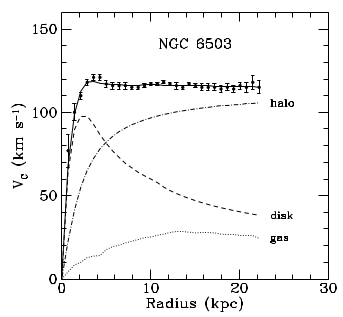
\includegraphics[width=0.5\linewidth]{images/Rotation Curve.png}
    \caption{Rotation curve of NGC 6503. The dotted, dashed, and dash-dotted lines are the contributions of gas, disk, and dark matter, respectively \cite{Bertone_2005}.}
    \label{Rotation Curve image}
\end{figure}
The existence of dark matter can be inferred from several types of evidence, the most compelling of which is the rotation curves of galaxies. According to the theory of Newtonian physics, the velocity of stars at any point of a galaxy should be proportional to the square root of the radius, or $1/\sqrt{r}$, as shown in \autoref{Newtonian velocity}. However, observations show that the stars at the edge of galaxies have similar linear velocities to those closer to the center as shown in \autoref{Rotation Curve image}, which suggests that there is more matter present than what we can observe

\begin{eqnarray}\label{Newtonian velocity}
    v(r) &=& \sqrt{\frac{GM(r)}{r}}.
\end{eqnarray}

At the time of discovery, there were two possibilities to explain this inconsistency with Newtonian physics. Either Newtonian physics is wrong, or Newtonian physics is right but something is missing. It would be tough for physicists to assume that Newtonian physics is wrong, or if it is, then almost all of the physics they were discovering would collapse in that time. That led them to consider the second possibility choice, the missing something in the rotation velocity equation, \autoref{Newtonian velocity}. If Newtonian physics is not wrong, then \autoref{Newtonian velocity} must be right also, which means the only parameter they had gone wrong is the mass of the galaxy. If the mass of the galaxy is wrong, then how wrong was it? From the observation, \autoref{Rotation Curve image}, The velocity of NGC 6503 is typically stable from the center of the galaxy to the edge of it. This means the part where the mass of the galaxy goes wrong is it was too low. That concluded that the galaxy, or indeed galaxies, have an invisible mass, which means it does not interact with the light or in other words, photons. With this conclusion, at least we can tell that it has no charge \cite{Bertone_2005}.

\subsection{Gravitational Lensing}
\begin{figure}[h]
    \centering
    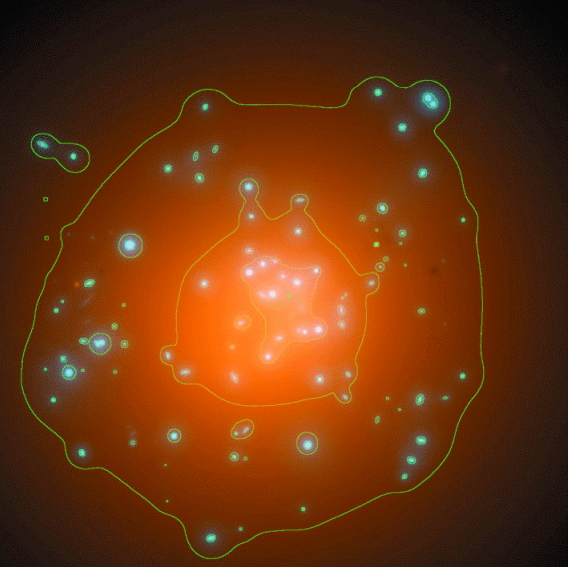
\includegraphics[width=0.5\linewidth]{images/Gravitational lensing.png}
    \caption{The galaxies around the galaxy cluster appear distorted and irregular due to insufficient mass for cluster formation \cite{Tyson_1998}.}
    \label{gravittional lensing}
\end{figure}
Another proof of the existence of dark matter and its affection for the surrounding object is gravitational lensing. We know that gravitational lensing is a phenomenon of the bending of space due to a strong field of gravity, in the case of dark matter, it also does. From the observation, since the first time, scientists found evidence of gravitational lensing in 1979 \cite{Walsh1979}, scientists have found more evidence of gravitational lensing, but in some areas of space, it appears to have concerns. For some reason, some areas of space appear to have an empty barrier to oppose any object from getting through it, also known as a dark halo, and it does affect surrounding areas like massive objects, course to gravitational lensing phenomena. This case is consistent with the fact that scientists found out that dark matter has no interaction with a photon. That is the reason we can believe more about the existence of dark matter in the universe. Moreover, this evidence reveals areas of possibility for finding dark matter. Since areas that are irregular or not consistent with the expected result, and have dark matter properties that do not interact with photons, we can assume the dark matter is usually in the areas of the dark halo.

\subsection{Bullet Cluster}
\begin{figure}[h]
    \centering
    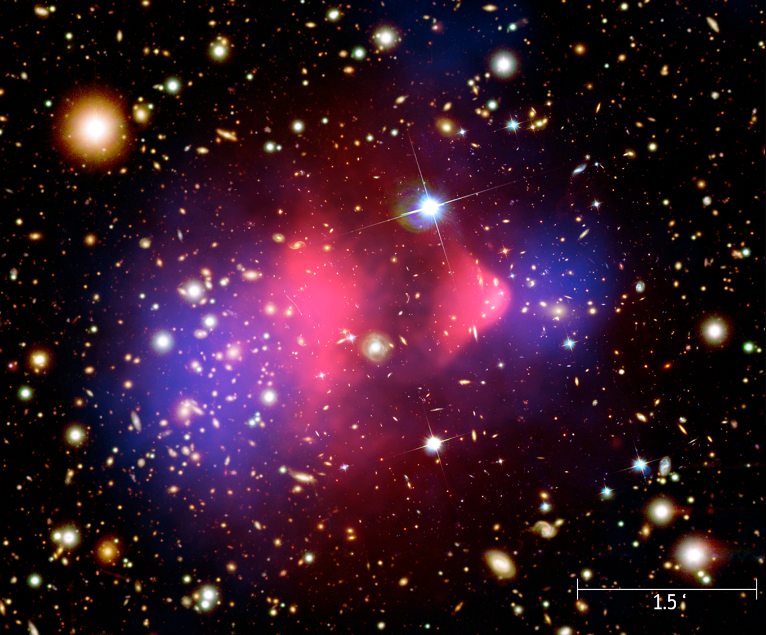
\includegraphics[width=0.5\linewidth]{images/bullet cluster.png}
    \caption{After the galaxies collided, a photo was taken of the resulting galaxy cluster. The red color represents the distribution of cloud gas observed through X-rays, while the blue color represents the mass distribution observed through gravitational lensing \cite{nasa_svs_2023}.}
    \label{fig: bullet cluster}
\end{figure}
Over time, scientists have developed various methods of observing the universe, such as using X-rays and taking advantage of the gravitational lensing phenomenon. X-ray observations provide information about the components in the observed areas that interact with light, which is the object that emits high-energy EM waves in the X-ray range. In \autoref{fig: bullet cluster}, we can see the collision of galaxy clusters. The red area represents the observation from X-rays, while the blue area represents the effect of the gravitational field and the cause of gravitational lensing phenomena. Due to the properties of dark matter, it was logical to assume that gravitational lensing in those areas with insufficient mass in \autoref{fig: bullet cluster} was caused by dark matter.

In \autoref{fig: bullet cluster}, we can see inconsistencies in the collisions of galaxy clusters. The blue area, which we suggest is dark matter, passes through another galaxy cluster easily, while the red area, which is a cloud of gas detected by X-ray observation and it is a baryon or matter we know from the periodic table of elements, does not seem to pass through each other easily and is left behind. If the blue area can pass through the other galaxy cluster and the red area cannot, then we can conclude that the blue area, which we suggest to be dark matter, is a weakly interacting matter.

\section{Dark Matter Candidates}
We have covered the characteristics of dark matter for three preferences in the previous section. Dark matter has three main properties: first, it has no interaction with light or photons, second, it has mass and can bend space because of a strong gravitational field, and third, it could have weak interactions because it hardly interacts with each other. When we consider everything, we can conclude that dark matter is not baryonic matter, which raises the question of what exactly dark matter is composed of. This section will address the potential candidates for dark matter by concentrating on known non-baryonic matter.

\subsection{Weakly Interacting Massive Particles (WIMPs)}
WIMPs are the most popular dark matter candidates because they fit well with our current understanding of physics \cite{Bertone_2018}. They are thought to be particles that interact with ordinary matter only through a weak nuclear force, which is very weak. This means that they would be very difficult to detect, but they would also be very stable, which is important for a dark matter candidate.
WIMPs are also thought to be massive, with masses ranging from GeV to TeV. This is based on the fact that dark matter is thought to comprise about 85\% of the matter in the universe, and WIMPs are hypothetical particles that are massive enough to account for this much matter.
Many experiments are searching for WIMPs, but none of them have yet produced a definitive detection. However, there have been some hints of WIMPs and scientists are hopeful that they will eventually be able to make a definitive detection.
\subsection{Axions}
Axions are a more exotic dark matter candidate \cite{bauer2018introduction}. They are thought to be particles that were first proposed to solve the strong CP problem in particle physics. The strong CP problem is a problem in quantum chromodynamics (QCD) \cite{Bertone_2018}, the theory of the strong force. QCD predicts that there should be a certain type of asymmetry in the universe, but this asymmetry is not observed. Axions were proposed as a way to solve this problem.
Axions are also thought to be very weakly interacting, but they are much lighter than WIMPs, with masses ranging from $\mu$eV to eV. This makes them even more difficult to detect than WIMPs.
\subsection{Sterile Neutrinos}
Sterile neutrinos are a hypothetical type of neutrino that does not interact with light or other forms of electromagnetic radiation. Neutrinos are known particles that are very weakly interacting, but they interact with light and other forms of electromagnetic radiation. Sterile neutrinos are thought to be even more weakly interacting than neutrinos, and they do not interact with light or other forms of electromagnetic radiation.
Sterile neutrinos can be heavier than WIMPs, with masses ranging from keV to GeV. This makes them more detectable than Axions, but they are still very difficult to detect. Some experiments are searching for sterile neutrinos, and there is some hope that they will eventually be able to find them.

\section{Dark Matter Detection}
There are two ways to detect dark matter in astrophysics.
\subsection{Direct Detection}
This involves setting up detectors that are sensitive to the interactions of dark matter particles with ordinary matter. If a dark matter particle collides with an atom in the detector, it can cause the atom to recoil, which can be detected.
\subsection{Indirect Detection}
This involves looking for the products of dark matter annihilation or decay. For example, if dark matter particles annihilate, they can produce gamma rays or other forms of radiation that can be detected by telescopes.

\section{Dark Matter Distribution in the Galaxies}
We take into consideration several possibilities about the galactic dispersion of dark matter in the Milky Way. An established benchmark option inspired by N-body simulations is the Nirvana, Frank, and White (NFW) profile. A better fit to more recent numerical simulations is being found for the Einasto profile, which is somewhat larger than NFW at kpc scales and does not converge to a power law at the galactic center (GC). The shape parameter, $\alpha$, varies from simulation to simulation, but 0.17 seems to emerge as a central, fiducial value that we adopt. In contrast, cored profiles like the Burkert profile and the truncated Isothermal profile appear to conflict with the results of numerical models. These profiles may instead be more driven by observations of galactic rotation curves. Conversely, Moore and associates have previously discovered profiles that were steeper than NFW. When computing dark matter signals in the Milky Way, it is helpful to have the whole range of these options available, so long as a convergent determination of the actual dark matter profile is not achieved \cite{Marco_Cirelli_2011}. The functional forms of these profiles are:
\begin{equation}
\begin{aligned}\label{dark matter density}
    NFW&:& \rho(r)_{NFW} &= \rho_s \frac{r_s}{r}\left(1+\frac{r}{r_s}\right)^{-2}\\
    Einasto&:& \rho(r)_{Ein} &= \rho_s\exp\left(\-\frac{2}{\alpha}\left(\frac{r}{r_s}^\alpha-1\right)\right)\\
    Isothermal&:& \rho(r)_{iso} &= \frac{\rho_s}{1+(r/r_s)^2}\\
    Burkert&:& \rho(r)_{Bur} &= \frac{\rho_s}{(1+r/r_s)(1+(r/r_s)^2)}\\
    Moore&:& \rho(r)_{Moo} &= \rho_s\left(\frac{r_s}{r}^{1.16}\right)\left(1+\frac{r}{r_s}\right)^{-1.84}
\end{aligned}
\end{equation}

Which have the following parameters:

\begin{table}[h]
    \centering
    \begin{tabular}{|l|c|c|c|}
    \hline
    DM halo  & $\alpha$ & $r_s$(kpc) & $\rho_s$(GeV/cm$^3$)\\
    \hline
    NFW & - & 24.42 & 0.184\\
    Einasto & 0.17 & 28.44 & 0.033\\
    EinastoB & 0.11 & 35.24 & 0.021\\
    Isothermal & - & 4.38 & 1.387\\
    Burkert & - & 12.67 & 0.712\\
    Moore & - & 30.28 & 0.105\\
    \hline
    \end{tabular}
    \caption{The parameters used to fill dark matter density from various profiles \cite{Marco_Cirelli_2011}.}
    \label{tab: paremeters}
\end{table}

Since the NFW profile is the most widely used and conventional one for explaining the dark matter distribution in the universe, we will employ it in this research.
\begin{figure}
    \centering
    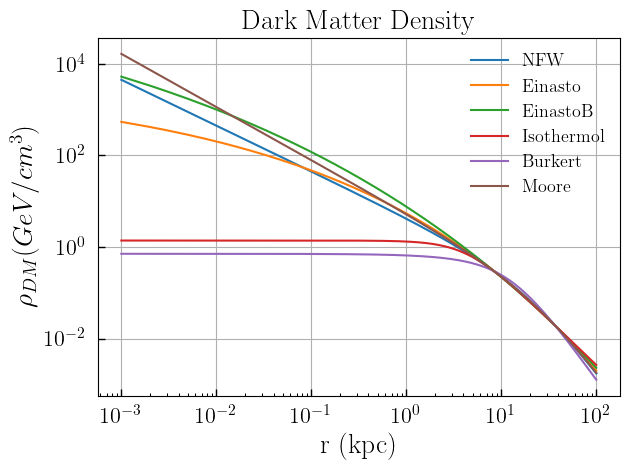
\includegraphics[width=0.6\linewidth]{images/Dark Matter Density.png}
    \caption{Dark matter density profiles}
    \label{fig: DM density}
\end{figure}

\section{Portal Dark Matter Model}
A portal dark matter model \cite{Pongkitivanichkul:2019cvm} is a type of dark matter model that proposes that dark matter interacts with ordinary matter through a mediator particle. The portal dark matter model is a general framework that can accommodate a wide variety of dark matter candidates. The specific properties of the mediator particle and the dark matter particle will depend on the specific model.
One of the most popular portal dark matter models is the WIMP (weakly interacting massive particle) model. In the WIMP model, the mediator particle is a new boson called the WIMPzilla. The WIMPzilla is a very massive particle, and it interacts with ordinary matter through a weak nuclear force.
Another popular portal dark matter model is the axion model. In the axion model, the mediator particle is a new pseudoscalar particle called the axion. The axion is a very light particle, and it interacts with ordinary matter through a strong force \cite{Klangburam:2021vli}.
Portal dark matter models are a promising approach to dark matter research. They are flexible enough to accommodate a wide variety of dark matter candidates, and they are testable by experiments. Generally, the Lagrangian of the model in this class is given by
\begin{equation}\label{DM model}
	\begin{split}
		\mathcal{L}&=(D_\mu H)^\dagger(D^\mu H)+\frac{1}{2}(\partial_\mu\Phi)(\partial^\mu\Phi)+\mu^2H^\dagger H-\lambda(H^\dagger H)^2+\frac{\mu^2_\phi}{2}\Phi^2-\frac{\lambda_\phi}{2}\Phi^4\\&-\frac{\lambda_\phi H}{2}\Phi^2 H^\dagger H+\lambda_\chi\phi\chi\chi,
	\end{split}
\end{equation}

\begin{tabbing}
    \indent\= \indent\= \indent\= \indent\= \indent\=\\
    where:
    \>\>\> $H$ \> $\equiv$ Higgs field,\\
    \>\>\> $\chi$ \>$\equiv$ Dark matter field,\\
    \>\>\> $\Bar{\chi}$ \> $\equiv$ Anti-dark matter field.
\end{tabbing}

\noindent In this research, we are considering the dark matter annihilation process as

\begin{equation*}
    \chi\Bar{\chi} \longrightarrow \phi_1\phi_2 \longrightarrow j\Bar{j} + j'\Bar{j'},
\end{equation*}

\begin{tabbing}
    \indent\= \indent\= \indent\= \indent\= \indent\= \indent\= \indent\= \\
    where:
    \>\>\> $\phi_1$ and $\phi_2$ \>\>\>$\equiv$ \> Mediator particle,\\
    \>\>\> $j$ and $\Bar{j}$ \>\>\>$\equiv$ \> Particle in the standard model and itself anti-matter respectively,\\
    \>\>\> $j'$ and $\Bar{j'}$ \>\>\>$\equiv$ \> Particle in the standard model and itself anti-matter respectively but\\ \>\>\>\>\>\> in the opposite direction of $j\Bar{j}$.
\end{tabbing}

\begin{figure}
    \centering
    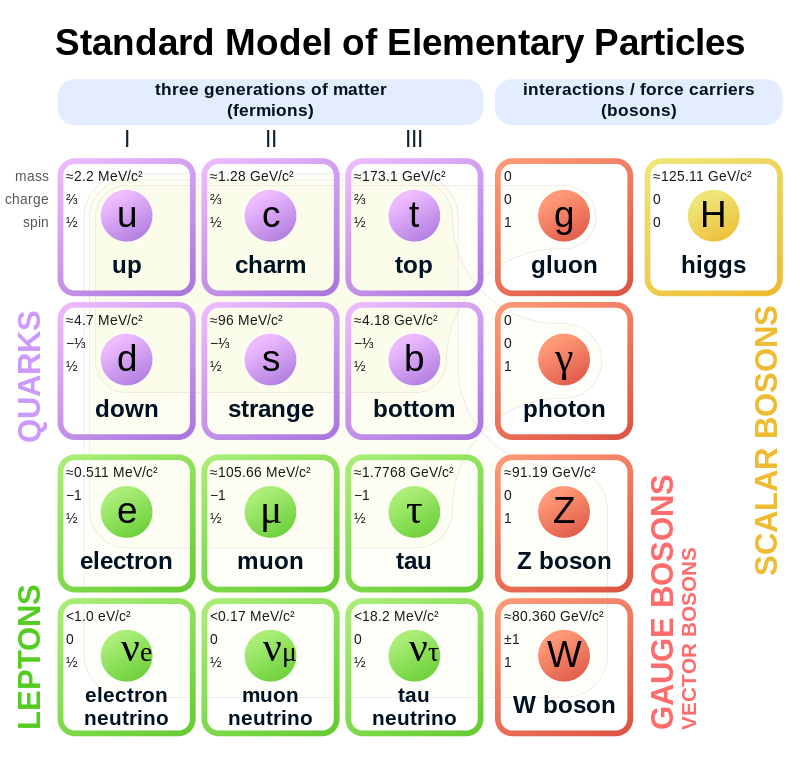
\includegraphics[width=\linewidth]{images/Standard_Model_of_Elementary_Particles.png}
    \caption{A table describes the properties of particles in the standard model of elementary particles \cite{enwiki:1199429080}.}
    \label{fig: standard model}
\end{figure}


\begin{figure}
    \centering
    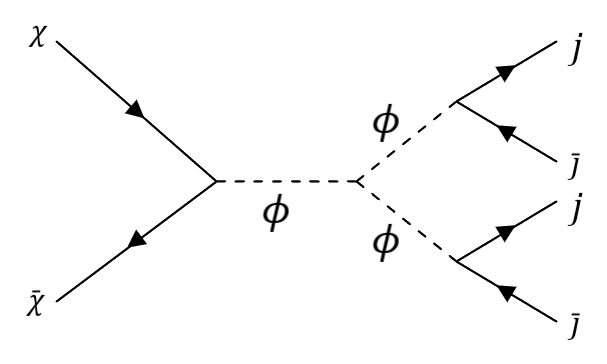
\includegraphics[width=0.5\linewidth]{images/feynman.png}
    \caption{Feyman diagram of dark matter annihilation process in the portal dark matter model.}
    \label{fig:enter-label}
\end{figure}
\section{Fermi-LAT gamma-ray Excess}
This is an excess of gamma-ray observed by the Fermi Large Area Telescope (Fermi-LAT) in the direction of the Galactic center. The excess was first reported in 2012 and was confirmed by subsequent observations. The excess is seen at energies between 1 and 100 GeV. It is not well-explained by known astrophysical sources, such as supernova remnants or pulsars. Our primary hypothesis posits that the observed excess originates from dark matter particle annihilation.

The Fermi-LAT gamma-ray excess is consistent with the expected spectrum of gamma rays from dark matter annihilation. The excess is also consistent with the expected spatial distribution of dark matter in the Milky Way. The excess is not yet a definitive detection of dark matter, but it is a promising dark matter candidate. More data is needed to confirm the origin of the excess, but it is an exciting development in the search for dark matter.

\begin{figure}[h]
	\centering
	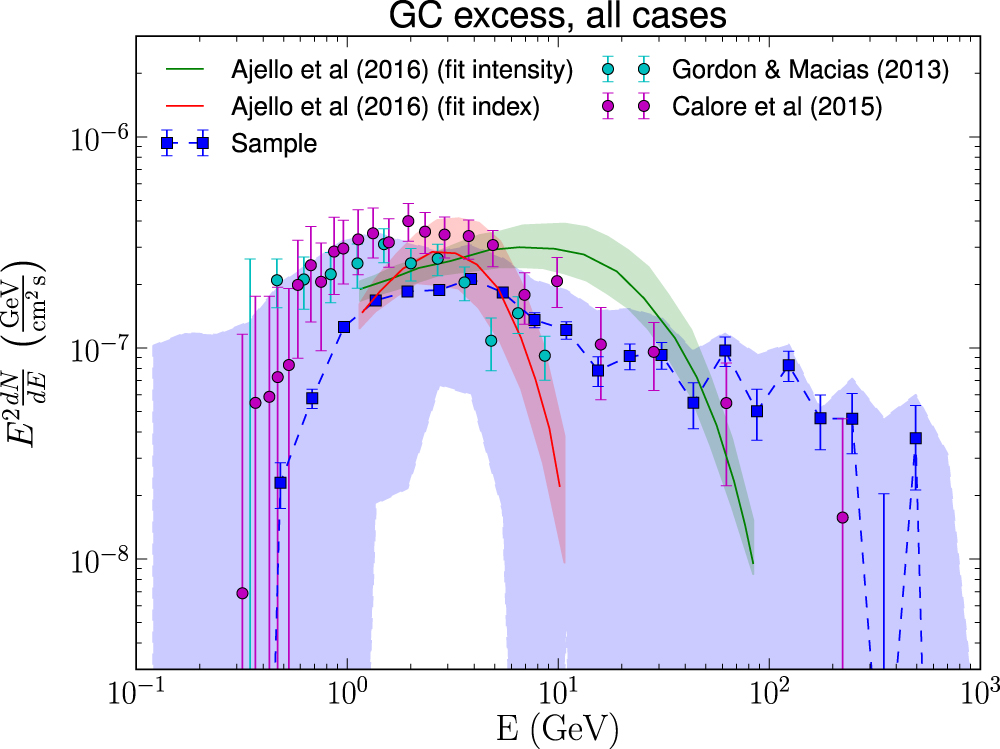
\includegraphics[width=0.7\linewidth]{images/Fermi-LAT}
	\caption{The Fermi GC GeV Excess and Implications for Dark Matter \cite{Ackermann_2017}.}
	\label{fig:fermi-lat}
\end{figure}

\begin{figure}
    \centering
    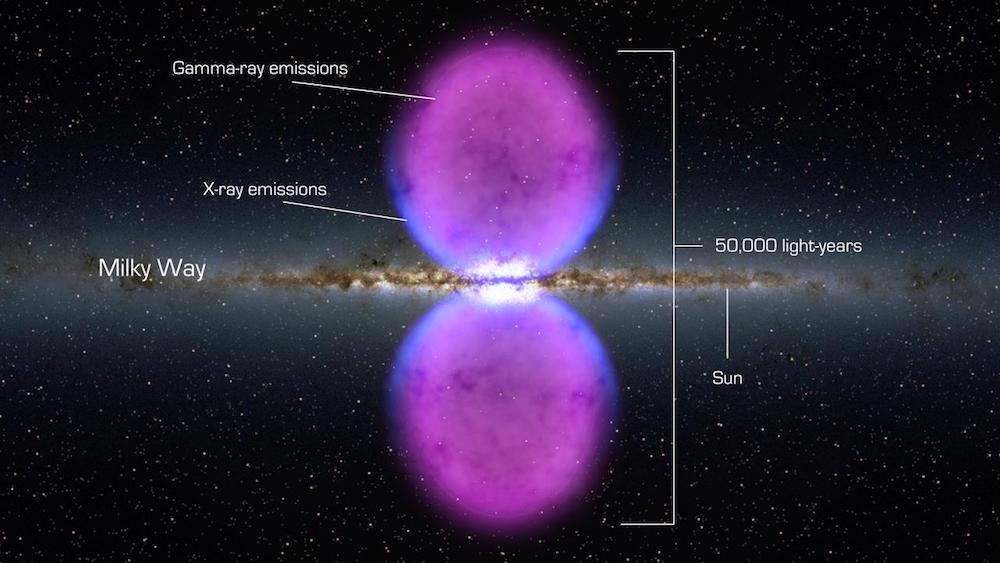
\includegraphics[width=0.5\linewidth]{images/Buble of gamma-ray.jpg}
    \caption{Image represents the mysterious gamma-ray performed in a bubble-like form \cite{alvarezhurtado2019correlation}.}
    \label{fig: Bubble of gamma-ray}
\end{figure}

\section{J-factors}
The J-factor is an important instrument in dark matter detection research. It is a method of measuring the quantity of dark matter that is present in a target astronomical object, such as a star cluster or dwarf galaxy, along a certain focal length. The J-factor indicates the amount of annihilation or decay products from dark matter that we might be able to find while observing a particular astronomical object.\\
\indent Beyond merely a numerical value, the J-factor captures the complex connection between particle physics and astrophysical modeling in the search for dark matter. Accurate modeling of the gravitational dynamics of astronomical objects, such as dwarf galaxies, which are believed to be dominated by dark matter, is necessary to understand the distribution of dark matter inside them. In turn, this gives the framework for determining the predicted signal intensity and the J-factor for different cases of dark matter decay or annihilation.\\
\indent Essentially the J-factor guides scientists in their ceaseless search for this unexplained cosmic component by acting as a link between the observable universe and the mysterious world of dark matter \cite{Marco_Cirelli_2011}. The equation expresses the relation of the J-factor and the line of sign, (l.o.s.), shown in \autoref{J-factor}.
\begin{eqnarray}\label{J-factor}
    J\left(\psi\right) = \frac{1}{R_{sc}\rho_{sc}} \int_{l.o.s.} \rho\left(r\right) \,dr
\end{eqnarray}
\begin{tabbing}
    \indent\= \indent \= \indent \= \indent \= \indent\= \\
    Where:
    \>\>\> $\psi$ \> = \> Solid angle from the Earth to the area of annihilation,\\
    \>\>\> $R_{sc}$ \> = \> Radius of the Solar System,\\
    \>\>\> $\rho_{sc}$ \> = \> Density of dark matter in the Solar System,\\
    \>\>\> $r$ \> = \> Radius from the center of the Milky Way to the area of annihilation.\\
\end{tabbing}

\chapter{Methodology}
\section{Creating Spectrum from Dark Matter Portal Model}
\subsection{Retrieve Data from the Dark Matter Portal Model}
We use data from two software, \textbf{\textit{CascadeSpectra}}  \cite{Marco_Cirelli_2011} and \textbf{\textit{HDMSpectra}} \cite{Bauer_2021}, which simulate the flux of gamma rays produced after the annihilation of dark matter. Our research focuses on examining the gamma-ray flux produced from various channels of elementary particles, such as $m_\chi m_\chi \rightarrow d, u, s, c, b, t, e, \mu, \tau,  g, Z, W$, and $h$.

The file we used, \textbf{\textit{CascadeSpectra}}, can be downloaded by clicking the \textbf{Download} button on the last line of \autoref{PPPC4DMID}. This code allows us to simulate dark matter annihilation not only for gamma rays but also for other standard model particles. For our research, we used the data named \textbf{AtProduction\_gammas.dat}, which contains most of the standard model particles that are annihilated from dark matter to gamma rays, except for the light quarks (up, down, and strange), which are labeled as ``q''. To avoid inconsistencies with \textbf{\textit{HDMSpectra}}, we changed the name of each particle in \textbf{ AtProduction\_gammas.dat} to match the names used in \textbf{\textit{HDMSpectra}}. The data we obtained was in the form of$dN/dx$, where x is $2E/m_\chi$. However, this format was not suitable for our purposes, so we converted it into the following of $dN/dE$ using the following methods.

\begin{eqnarray}
\begin{aligned}
	\frac{dN}{dx} &= \frac{dN}{d\frac{2E}{m_\chi}} \\
	&= \frac{m_\chi}{2} \frac{dN}{dE} \\
	\frac{dN}{dE} &= \frac{2}{m_\chi} \frac{dN}{dx}
 \label{factor}
 \end{aligned}
\end{eqnarray}

\begin{figure}
	\centering
	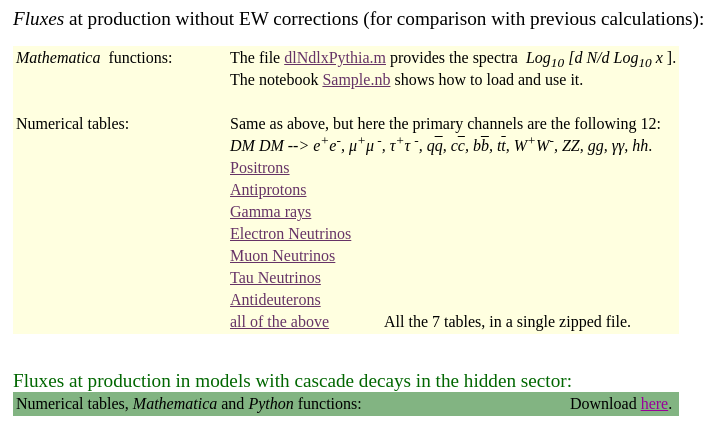
\includegraphics[width=0.75\linewidth]{images/PPPC4DMID.png}
	\caption{The source of \textbf{\textit{CascadeSpectra}} codes \cite{Marco_Cirelli_2011} which we use to simulate the flux of gamma-ray from dark matter annihilation.}
	\label{PPPC4DMID}
\end{figure}

For \textbf{\textit{HDMSpectra}}, we downloaded it from the website \url{https://github.com/nickrodd/HDMSpectra} \cite{Bauer_2021}. Similar to \textbf{\textit{CascadeSpectra}}, we need to apply a factor to convert it from $dN/dE$ to $dP/dE$, as shown in \autoref{factor}.

We use both \textbf{\textit{CascadeSpectra}} and \textbf{\textit{HDMSpectra}} in our research because we believe \textbf{\textit{HDMSpectra}} provides more accurate results for high-mass dark matter, which is our main objective. However, \textbf{\textit{HDMSpectra}} has a minimum mass limit of 500 GeV, while the Fermi-LAT reference data starts at about 0.5 GeV, which is within the range covered by \textbf{\textit{CascadeSpectra}}.

\begin{figure}
    \centering
    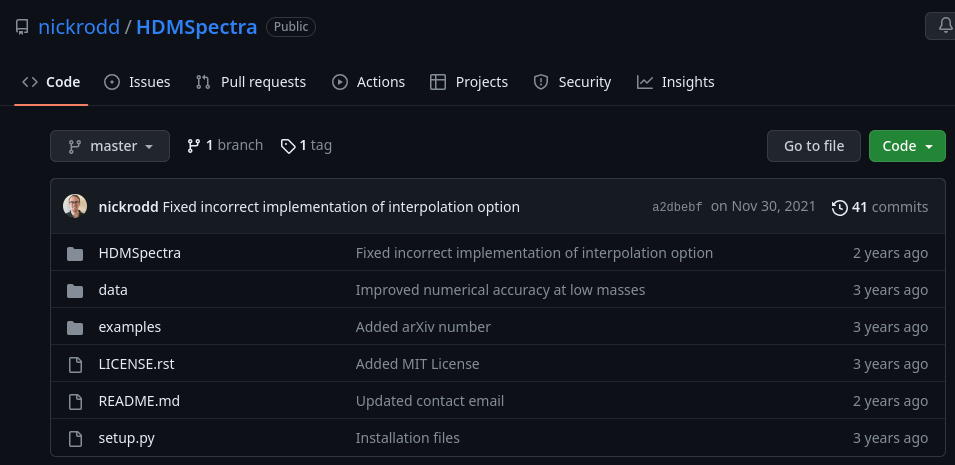
\includegraphics[width=0.75\linewidth]{images/HDMSpectra_source.png}
    \caption{A source of HDMSpectra Python codes \cite{Bauer_2021}.}
    \label{HDMSpectra-source}
\end{figure}

\subsection{Find the Probability of Finding Gamma-ray Flux from Various Dark Matter Mass Annihilation}
In the previous section, we explained how to retrieve data on the flux of gamma rays emitted from the annihilation of dark matter. To determine the probability of this occurrence per unit of energy, we need to explore a wide range of possibilities for dark matter mass in the field of our interest. In this case, we do not know what scope of the range will give us the best-fit data, so we need to find it from the least mass that \textbf{\textit{CascadeSpectra}} and \textbf{\textit{HDMSpectra}} can reproduce Due to those reasons, we decided to vary the dark matter mass from 5 GeV to 1000 TeV. However, the data we obtain is still unusable because we need to determine only the point that consists of the data from Fermi-LAT, which starts at 0.5 GeV and ends at 500 GeV by approximation. To do that, we use a numerical method called interpolation, which allows us to find the approximate value of data from a discrete sample set of data and create a function that can give us a value of that data in the specific variable that those functions relate to, as shown in \autoref{fig:dPdE_sample}.

The reason behind the pick-up of two simulations and combining them is that \textbf{\textit{CascadeSpectra}} is untrustable at high-mass dark matter mass, which is the scope of this research interest. At the same time, \textbf{\textit{HDMSpectra}} allows us to simulate the flux of gamma-ray from dark matter annihilation above 500 GeV, but the sample data we define as comparing or real data from Fermi-LAT begins at 0.5 to 500 GeV, as mentioned before. So we decided to combine those models and lay a condition that, if the mass of dark matter is less than 500 GeV, simulate the flux from \textbf{\textit{CascadeSpectra}}, and on the other hand, if the dark matter mass is above 500 GeV, use the \textbf{\textit{HDMSpectra}} instead.

\begin{figure}
	\centering
	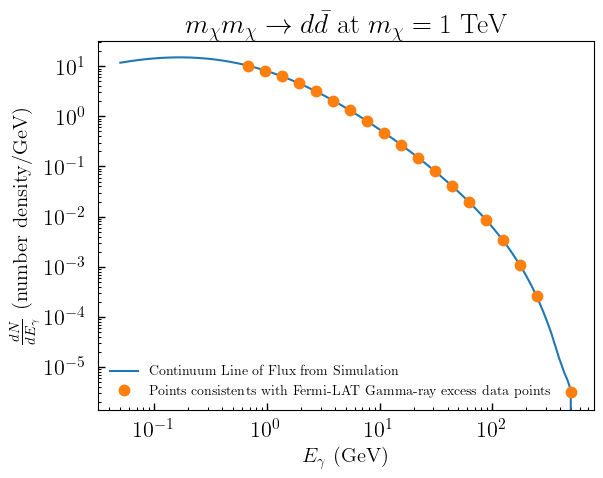
\includegraphics[width=0.75\linewidth]{images/dPdE_sample_2}
	\caption{A graph is a representation of the simulated spectrum of the flux of gamma-ray energy per gamma-ray energy from the annihilation of dark matter at 7,100 GeV mass in the d-quark channel. }
	\label{fig:dPdE_sample}
\end{figure}

\section{Calculation of J-factors}%Derive J-Factor - I have done it%
\begin{figure}
    \centering
    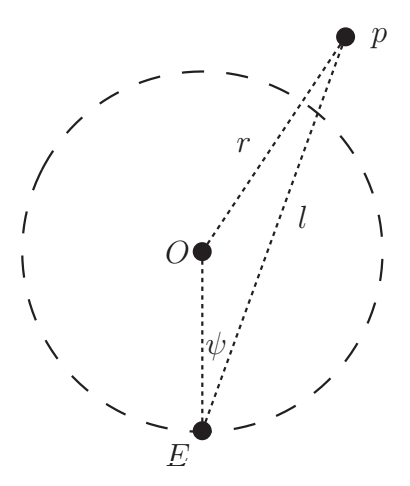
\includegraphics[width=0.3\linewidth]{images/distance.PNG}
    \caption{This simplified sketch represents the estimated distribution of dark matter in the Milky Way galaxy. The Earth's location is marked by $E$, the galactic center by $O$, and several possible locations of dark matter by $p$.}
    \label{fig: distance}
\end{figure}
J-factor is a factor that we implied every parameter related to astronomy within it, in this research, it is the factor that refers to the distance from here, Earth, to the center of the Milky Way galaxy, in particular, it was shown in \autoref{J-factor}

From the \autoref{fig: distance} we can find the relation between the radius from the center of the Milky Way to the area of annihilation and the distance from the Earth to the area of annihilation as

\begin{equation}\label{r}
	r=\sqrt{R_{sc}^2+l^2-2R_{sc}l\cos(\psi)}.
\end{equation}

\noindent If we consider the longest distance in the Milky Way, we will have

\begin{equation}\label{Rmw}
    R_{MW}=\sqrt{R_{sc}^2+l_{max}^2-2R_{sc}l_{max}\cos(\psi)},
\end{equation}

\begin{tabbing}
    \indent \= \indent \= \indent \= \indent \= \indent\= \indent\= \\
    where:
    \>\>\> $R_{MW}$ \>\> $\equiv$ \> Radius of the Milky Way galaxy,\\
    \>\>\> $l_{max}$ \>\> $\equiv$ \> Distance from the Earth to the area of annihilation,\\
    \>\>\> $\Psi$ \>\> $\equiv$ \> Angle from the Earth to the area of annihilation. 
\end{tabbing}
where $R_{MW}$ is the radius from the center of the Milky Way to the longest distance that allows the annihilation of dark matter in the Milky Way.\\
Rearrange \autoref{Rmw}, we obtain the term of the longest distance from the Earth to the area of dark matter annihilation.

\begin{eqnarray}\label{lmax}
    l_{max} &=& \sqrt{R_{MW}^2-R_{sc}^2\sin^2(\psi)}+R_{sc}\cos(\psi)
\end{eqnarray}
Then we will integrate over the line of sight(l.o.s.), and solid angle, and substitute \autoref{dark matter density}, in the part of NFW profile into \autoref{J-factor}, we obtain

\begin{equation}
	J=\frac{1}{R_{sc}\rho_{sc}^2}\int_{0}^{4\pi}\int_{0}^{l{max}}\rho_s \frac{r_s}{r}\left(1+\frac{r}{r_s}\right)^{-2}drd\Omega
\end{equation}

where $\frac{1}{R_{sc}\rho_{sc}^2}$ is the normalization factor that cancels the dimension of the J-factor.
\begin{figure}
	\centering
	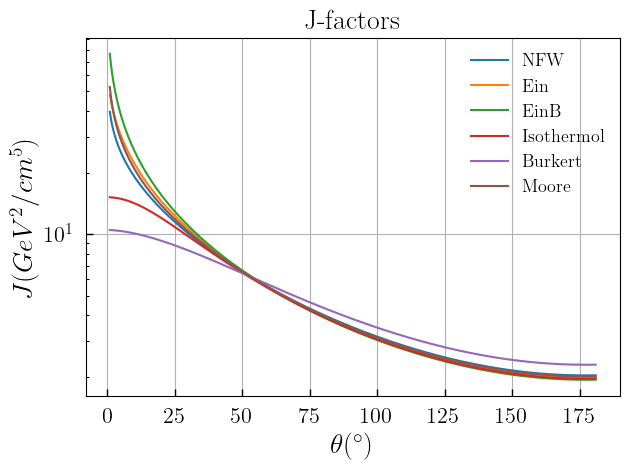
\includegraphics[width=0.75\linewidth]{images/J-factors.png}
	\caption{J-factors of dark matter from various dark matter profiles.}
	\label{J-factor fig}
\end{figure}

\section{Calculating the Probability of Finding a Particle $j$ with Energy $E_j$}
From the solid angle, $d\Omega$, we can find the probability of finding particles $j$ at azimuthal angle, $\theta$  \cite{Klangburam:2021vli} as
\begin{equation}
\begin{aligned}
    dP &\propto \int_{\phi=0}^{2\pi}d\Omega \propto 2\pi\sin(\theta)\\
    \frac{dP}{d\theta} &\propto 2\pi\sin(\theta)\\
    \int_{\theta =0}^{\pi}\frac{dP}{d\theta}d\theta &= 2\pi N[-\cos(\theta)]\Big|_{\theta = 0}^\pi\\
    &= 1.\\
    N &= \frac{1}{4\pi}
\end{aligned} 
\end{equation}
Which mean
\begin{equation}
\begin{aligned}
    \frac{dP}{d\theta} &= \frac{1}{2}\cdot\sin(\theta).\\
\end{aligned}
\end{equation}
From \cite{Klangburam:2021vli}, we know that
\begin{equation}\label{Energy j}
\begin{aligned}
    E_j &= \frac{m_\chi}{2}(1+\lambda_\phi\lambda_j\cos(\theta)),\\
\end{aligned}    
\end{equation}
where
\begin{equation}\label{lambda_phi_j}
\begin{aligned}
    \lambda_\phi &= \sqrt{1-(m_\phi/m_\chi)^2}\\
    \lambda_j &= \sqrt{1-(2m_j/m_\phi)^2}.
\end{aligned}
\end{equation}
Then we rearrange \autoref{Energy j}, we obtain
\begin{equation}
\begin{aligned}
    \cos(\theta) &= \frac{1}{\lambda_\phi\lambda_j}\left(\frac{2E_j}{m_\chi}-1\right),\\
    \sin(\theta) &= \frac{1}{\lambda_\phi\lambda_j} \sqrt{\lambda_\phi^2\lambda_j^2 - \left(\frac{2E_j}{m_\chi}-1\right)^2},
\end{aligned}
\end{equation}
which make
\begin{eqnarray}
    \frac{dP}{d\theta} = \frac{1}{2\lambda_\phi\lambda_j} \sqrt{\lambda_\phi^2\lambda_j^2 - \left(\frac{2E_j}{m_\chi}-1\right)^2}.
\end{eqnarray}
Since a particle with angle $\theta$ is proportional to the particle with energy, $E_j$, in other words, we have obtained the probability of finding a particle with energy, $E_j$.
\begin{eqnarray}
    \frac{dP}{dE_j} \propto \frac{1}{2\lambda_\phi\lambda_j} \sqrt{\lambda_\phi^2\lambda_j^2 - \left(\frac{2E_j}{m_\chi}-1\right)^2}.
\end{eqnarray}
Next, we need to normalize the probability to 1: 
\begin{eqnarray}\label{integral prop}
    \int_{E_{min}}^{E_{max}} \frac{dP}{dE_j}dE_j &=& 1\\
    \int_{E_{min}}^{E_{max}} \frac{N}{2\lambda_\phi\lambda_j} \sqrt{\lambda_\phi^2\lambda_j^2 - \left(\frac{2E_j}{m_\chi}-1\right)^2}dE_j &=& 1,
\end{eqnarray}
where $N$ is the parameter we add to complete the proportional to the equation.
From \autoref{Energy j}, we can find the maximum and minimum energy of particle $j$ by considering the $\cos$ property as shown in 
\begin{equation}
\begin{aligned}
    \cos(\pi) &=& -1\\
    \cos(2\pi) &=& 1.
\end{aligned}
\end{equation}
That means we obtain
\begin{equation}\label{Emin Emax}
\begin{aligned}
    E_{j, min} &=& \frac{m_\chi}{2}(1-\lambda_\phi\lambda_j)\\
    E_{j, max} &=& \frac{m_\chi}{2}(1+\lambda_\phi\lambda_j).
\end{aligned}
\end{equation}
Substitute \autoref{Emin Emax} into \autoref{integral prop}
\begin{eqnarray}\label{integral prop with boundary}
    \int_{\frac{m_\chi}{2}(1-\lambda_\phi\lambda_j)}^{\frac{m_\chi}{2}(1+\lambda_\phi\lambda_j)} \frac{N}{2\lambda_\phi\lambda_j} \sqrt{\lambda_\phi^2\lambda_j^2 - \left(\frac{2E_j}{m_\chi}-1\right)^2}dE_j &=& 1.
\end{eqnarray}
Rearrange \autoref{integral prop with boundary}, we have
\begin{equation}
\begin{aligned}
    \frac{1}{N} &= \int_{\frac{m_\chi}{2}(1-\lambda_\phi\lambda_j)}^{\frac{m_\chi}{2}(1+\lambda_\phi\lambda_j)} \frac{1}{2\lambda_\phi\lambda_j} \sqrt{\lambda_\phi^2\lambda_j^2 - \left(\frac{2E_j}{m_\chi}-1\right)^2}dE_j\\
    &= \frac{m_\chi}{4\Lambda}\int_{\frac{m_\chi}{2}(1-\Lambda)}^{\frac{m_\chi}{2}(1+\Lambda)}\sqrt{\Lambda^2-\left(\frac{2E_j}{m_\chi}-1\right)^2}d\left(\frac{E_j}{m_\chi}-1\right)\\
    &= \frac{m_\chi\pi\Lambda}{8}.\\
\end{aligned}
\end{equation}
Note that $dE_j = \frac{m_\chi}{2}d\left(\frac{2E_j}{m_\chi}-1\right)$, and $\Lambda=\lambda_\phi \lambda_j$. Now we have obtained the complete parameter $N$
\begin{eqnarray}
    N &=& \frac{8}{m_\chi\pi\lambda_\phi\lambda_j}.
\end{eqnarray}
This leads us to the final solution of the probability of finding a particle from  energy, $E_j$
\begin{equation}\label{complete dPdE}
\begin{aligned}
    \frac{dP}{dE_j} &= \frac{\frac{8}{m_\chi\pi\lambda_\phi\lambda_j}}{2\lambda_\phi\lambda_j}\sqrt{\lambda_\phi^2\lambda_j^2-\left(1-\frac{2E_j}{m_\chi}\right)^2}\\
    &= \frac{4}{m_\chi\pi}\cdot\frac{1}{\lambda_\phi\lambda_j}\sqrt{\lambda_\phi^2\lambda_j^2-\left(1-\frac{2E_j}{m_\chi}\right)^2}.
\end{aligned}
\end{equation}

\section{Calculating the Gamma-ray Flux Produced from Dark Matter Annihilation}
To calculate the gamma-ray flux generated from the annihilation of dark matter and decay of mediators, we need to combine three important factors: \autoref{complete dPdE}, \autoref{Emin Emax}, and data on the probability of finding dark matter per gamma-ray energy for each dark matter mass into \autoref{dNdE}. These numbers represent the number of gamma-rays produced from each mediator and $j$ particle after the annihilation of dark matter per energy. The source for this information is \cite{Klangburam:2021vli}.
\begin{eqnarray}\label{dNdE}
    \left(\frac{dN}{dE}\right)_{\phi_1\phi_2}=\int_{E_{min}}^{E_{max}}\left(\frac{dP}{dE_\gamma}\right)_{j\bar{j}}\left(\frac{dP}{dE_j}\right)_{\phi_1}dE_j + \left(\frac{dP}{dE_\gamma}\right)_{j\bar{j'}}\left(\frac{dP}{dE_{j'}}\right)_{\phi_2}dE_{j'}.
\end{eqnarray}
By combining \autoref{dNdE} with \autoref{dPhidE} \cite{Klangburam:2021vli}, we can calculate the flux of gamma-rays per energy from the annihilation of dark matter particles.
\begin{eqnarray}\label{dPhidE}
	\frac{d\Phi}{dE_\gamma}=\frac{\left\langle\sigma\nu\right\rangle}{8\pi}\frac{R_{sc}\rho_{sc}^2}{m_\chi^2}J\left(\frac{dN}{dE}\right)_{\phi_1\phi_2}.
\end{eqnarray}
In the context of the research, we need to perform the flux of gamma-ray per gamma-ray energy from dark matter annihilation, and we already have almost all the necessary parameters except for the average value of cross-section, denoted by $\left<\sigma v\right>$. We have decided to leave this parameter as a free parameter and determine its value by using a computer to find the best-fit parameter. The process of finding the best-fit parameter will be discussed in detail in \autoref{Finding the Best Fit Parameters For Fermi-LAT Data}.

\section{Finding the Best Fit Parameters for Fermi-LAT Data} \label{Finding the Best Fit Parameters For Fermi-LAT Data}
To find the best-fit parameter, we aim to use the reduced chi-square as a method to represent the distribution of observed data from Fermi-LAT and the simulation we have obtained. Since we use the reduced chi-square as a tool to describe the distribution of the data, we use the minimization method to find the best-fit parameter to complete the missing part of this research. But at the same time, we know the gamma-rays from Fermi-LAT may not completely reproduce from the process of dark matter annihilation, it comes
to the idea of finding the unknown astronomical flux. The method of finding unknown astronomical flux is shown in \autoref{Finding unknown astronomy flux}, and the rest is to follow the same analysis to find the best-fit parameter again.

\section{Finding the Unknown Astronomical Flux}\label{Finding unknown astronomy flux}
In \cite{Folgado_2018}, the unknown astronomical flux was defined as an exponential function. Represent as
\begin{equation}
    \Phi_{astro} = NE_\gamma^{-\alpha}e^{-E_\gamma/E_{cut}}.
    \label{unknown astronomy flux equation}
\end{equation}
\begin{tabbing}
    \indent\= \indent\= \indent\= \indent\= \indent\= \indent\= \\
    Where:
    \>\>\> $\Phi_{astro}$ \>\>\> = Unknown astronomical flux,\\
    \>\>\> $E_\gamma$ \>\>\> = Excess gamma-ray energy detected by Fermi-LAT,\\
    \>\>\> $N, \alpha, E_{cut}$ \>\>\> = Free parameters.
\end{tabbing}
To improve the accuracy of our best-fit gamma-ray flux from the simulation, we can use an unknown astronomical flux. To do this, we can simply add the unknown astronomical flux into our main gamma-ray flux. The equation representing this process is as follows:
\begin{equation}
    \Phi = \Phi_{DM} + \Phi_{astro}
\end{equation}


\subsection{Finding Reduced chi-square}
By using the reduced chi-square equation, we can find the distribution of data from Fermi-LAT compared to our simulation.
\begin{equation}
\begin{aligned}
    \chi_\nu^2 &= \frac{\chi^2}{\nu}\\
	&= \sum_i\frac{O_i - C_i}{\sigma_i^2}
\end{aligned}
\end{equation}
when
\begin{equation}
    \nu = n-m
    \label{degree of freedom}
\end{equation}
\begin{tabbing}
    \indent\= \indent\= \indent\=\\
    where: \>\> $O$\> = The observed data,\\
    \>\> $C$\> = The calculated data,\\
    \>\> $\nu$\> = Degree of freedom,\\
    \>\> $n$\> = Number of observations,\\
    \>\> $m$\> = Number of fitted parameters.
\end{tabbing}
We need to calculate the reduced chi-square value for a given data set. The ideal reduced chi-square value is 1, but a value between 1-10 may also be acceptable, depending on the degree of freedom, as shown in \autoref{fig:chi-square-table}. If the reduced chi-square value is less than 1, it means the data is overfitting, which can cause problems if the observed data has errors. In such cases, the calculated data will also be incorrect, resulting in an inaccurate fit. Therefore, a reduced chi-square value greater than 1 is better. Once we have the reduced chi-square value, we can compare it with the chi-square table shown in \autoref{fig:chi-square-table} to determine the percentage point of the chi-square distribution.

\begin{figure}[h]
    \centering
    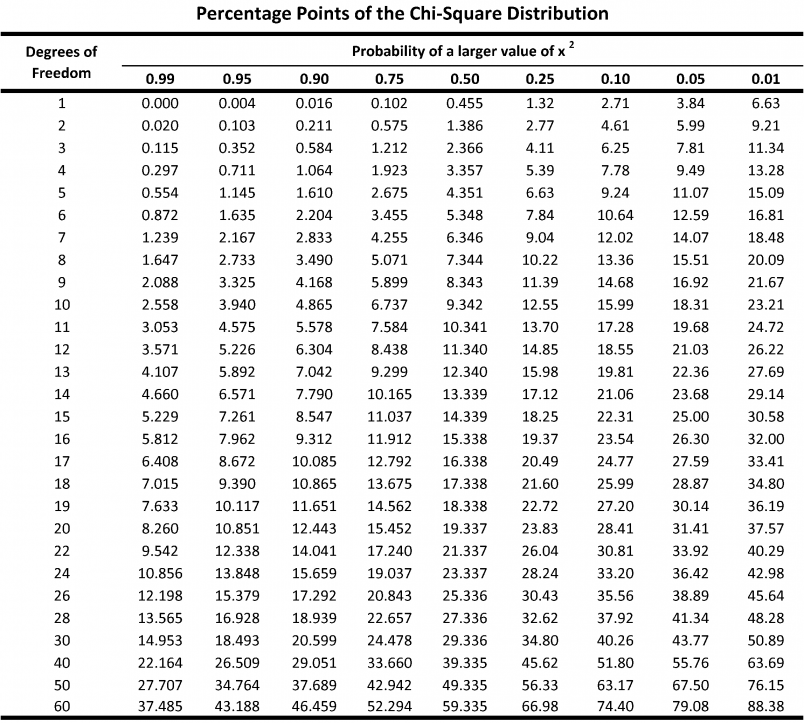
\includegraphics[width=\linewidth]{images/chi-square-table.png}
    \caption{The table of the percentage of the chi-square distribution \cite{passel}.}
    \label{fig:chi-square-table}
\end{figure}

\subsection{Minimization}
To determine the best-fit parameters, including the cross-section, $\left<\sigma v\right>$, and the dark matter mass, $m_\chi$, we utilize the Python module called \textbf{\textit{scipy}}. Within this module, there is a function called \textbf{\textit{bestfit}} which can help us find the best possible parameter that allows the experiment data and expected data to overlap. For this particular study, our parameters are $m_\chi$ and $\left<\sigma v\right>$, but we will only let the minimization function find the value of $\left<\sigma v\right>$.

This is because $m_\chi$ is not a parameter that can be arbitrarily set to any value; it must be within the scope of the data we have prepared, which in this research, is between 1 TeV and 100 TeV. Therefore, we need to use a loop to iterate over the range of $m_\chi$ values we have prepared and find the optimal $\left<\sigma v\right>$ value that provides the best fit between the experiment data and the expected data.

\subsection{Plotting a Contour Plot of Reduced chi-square}
To present the findings of the chi-square value and cross-section simply and understandably, we use contour plots. In this research, we use the $x$-axis to indicate the mass of dark matter, the $y$-axis for the cross-section, $\langle \sigma v \rangle$, and the $z$-axis as a contour to represent the chi-square value of these parameters. The contour plot is a good way to illustrate the constraints of dark matter mass and cross-section, which can simply represent the probability of finding dark matter based on mass and cross-section. We use this method to compare the simulation data and the simulation mixed with an unknown astronomical flux to show the significant improvement of the chi-square value from the result of the simulation data and the simulation mixed with an unknown astronomical flux.

%\subsection{Continuous Decaying From Scalar Mediator}

\chapter{Result and Discussion}
\section{Best-fit Graph and Contour Plot from the Simulation}
The simulation result was compared with the data from Fermi-LAT, and the best-fit parameters for the mass of dark matter, $m_\chi$, and cross-section, $\langle \sigma v \rangle$, were determined and presented in \autoref{tab: best fit}. However, in \autoref{fig: various DM}, the fit is not good, even though the best possible parameters are used. The $m_\chi$ column of \autoref{tab: best fit} shows that the fit is inconsistent since every particle has the best fit when $m_\chi$ is 1 or lower. This is because the lowest $m_\chi$ under our consideration is 1 TeV. Another proof of inconsistency is evident in the least $\chi^2$ column of \autoref{tab: best fit}. Although the chi-square value is the lowest, it still has a low confidence level, as shown in \autoref{fig:chi-square-table}.

\begin{table}[h]
    \centering
    \begin{tabular}{|c|c|c|c|}
        \hline
        Particles & $m_\chi$ (TeV) & $\langle\sigma v\rangle$($\times10^{-23}$ cm$^3$/s) & least $\chi^2$ \\
        \hline
         $d$ & 1.000 & 2.302 & 102.546\\
         $u$ & 1.000 & 2.308 & 102.319\\
         $s$ & 1.000 & 2.398 & 99.620\\
         $c$ & 1.000 & 2.268 & 101.792\\
         $b$ & 1.000 & 2.487 & 80.327\\
         $t$ & 1.000 & 4.398 & 38.756\\
         $e$ & 1.000 & 6.874 & 208.214\\
         $\mu$ & 1.000 & 1.766 & 207.510\\
         $\tau$ & 1.000 & 6.874 & 208.214\\
         $g$ & 1.000 & 2.749 & 64.610\\
         $Z$ & 1.000 & 3.647 & 70.123\\
         $W$ & 1.000 & 3.526 & 79.293\\
         $h$ & 1.000 & 3.389 & 43.069\\
         \hline
    \end{tabular}
    \caption{This table shows the result of the simulation of dark matter annihilation for quarks: $d, u,s,c,b,t$, leptons: $e, \mu, \tau$, and bosons: $g, Z, W, h$. The $m_\chi$ column shows the best possible dark matter mass to perform the best fit of the simulation and Fermi-LAT data under the scope of this research, from 1-100 TeV. The $\langle \sigma v \rangle$ shows the best possible cross-section. And the last column, least $\chi^2$ shows the lowest chi-square value from the simulation.}
    \label{tab: best fit}
\end{table}

In this simulation, we use 2 parameters, $m_\chi$ and $\langle \sigma v \rangle$, and the number of data points from Fermi-LAT is 19. By using the \autoref{degree of freedom}, our degree of freedom is 17, and from \autoref{fig:chi-square-table}, the confidence for a population variance or standard deviation at 90\% should be 10.085. Compared with the $\chi^2$ values we have, it shows us that the result from this simulation is far from acceptance.

In \autoref{fig: contour}, it shows the distribution of the chi-square value labeled with the color. As we can see, the least $\chi^2$ value shifts to the lower energy $m_\chi$, but in this research, the lowest energy of dark matter mass we consider is only 1 TeV, which does not allow us to see the lower mass consequence chi-square value. It does give us the trend of the chi-square value and also gives us a clue about what is missing. From the trend of gamma-ray flux from the simulation, we can assume that the gamma-ray flux produced from the annihilation of dark matter should be about the $1^{st}$ to the $11^{th}$ data point, and the rest comes from the unknown astronomical flux.

This leads us to the next section about discovering the value of parameters in \autoref{unknown astronomy flux equation} to fulfill the missing part of gamma-ray from this simulation.

\begin{figure}[h]
    \centering
    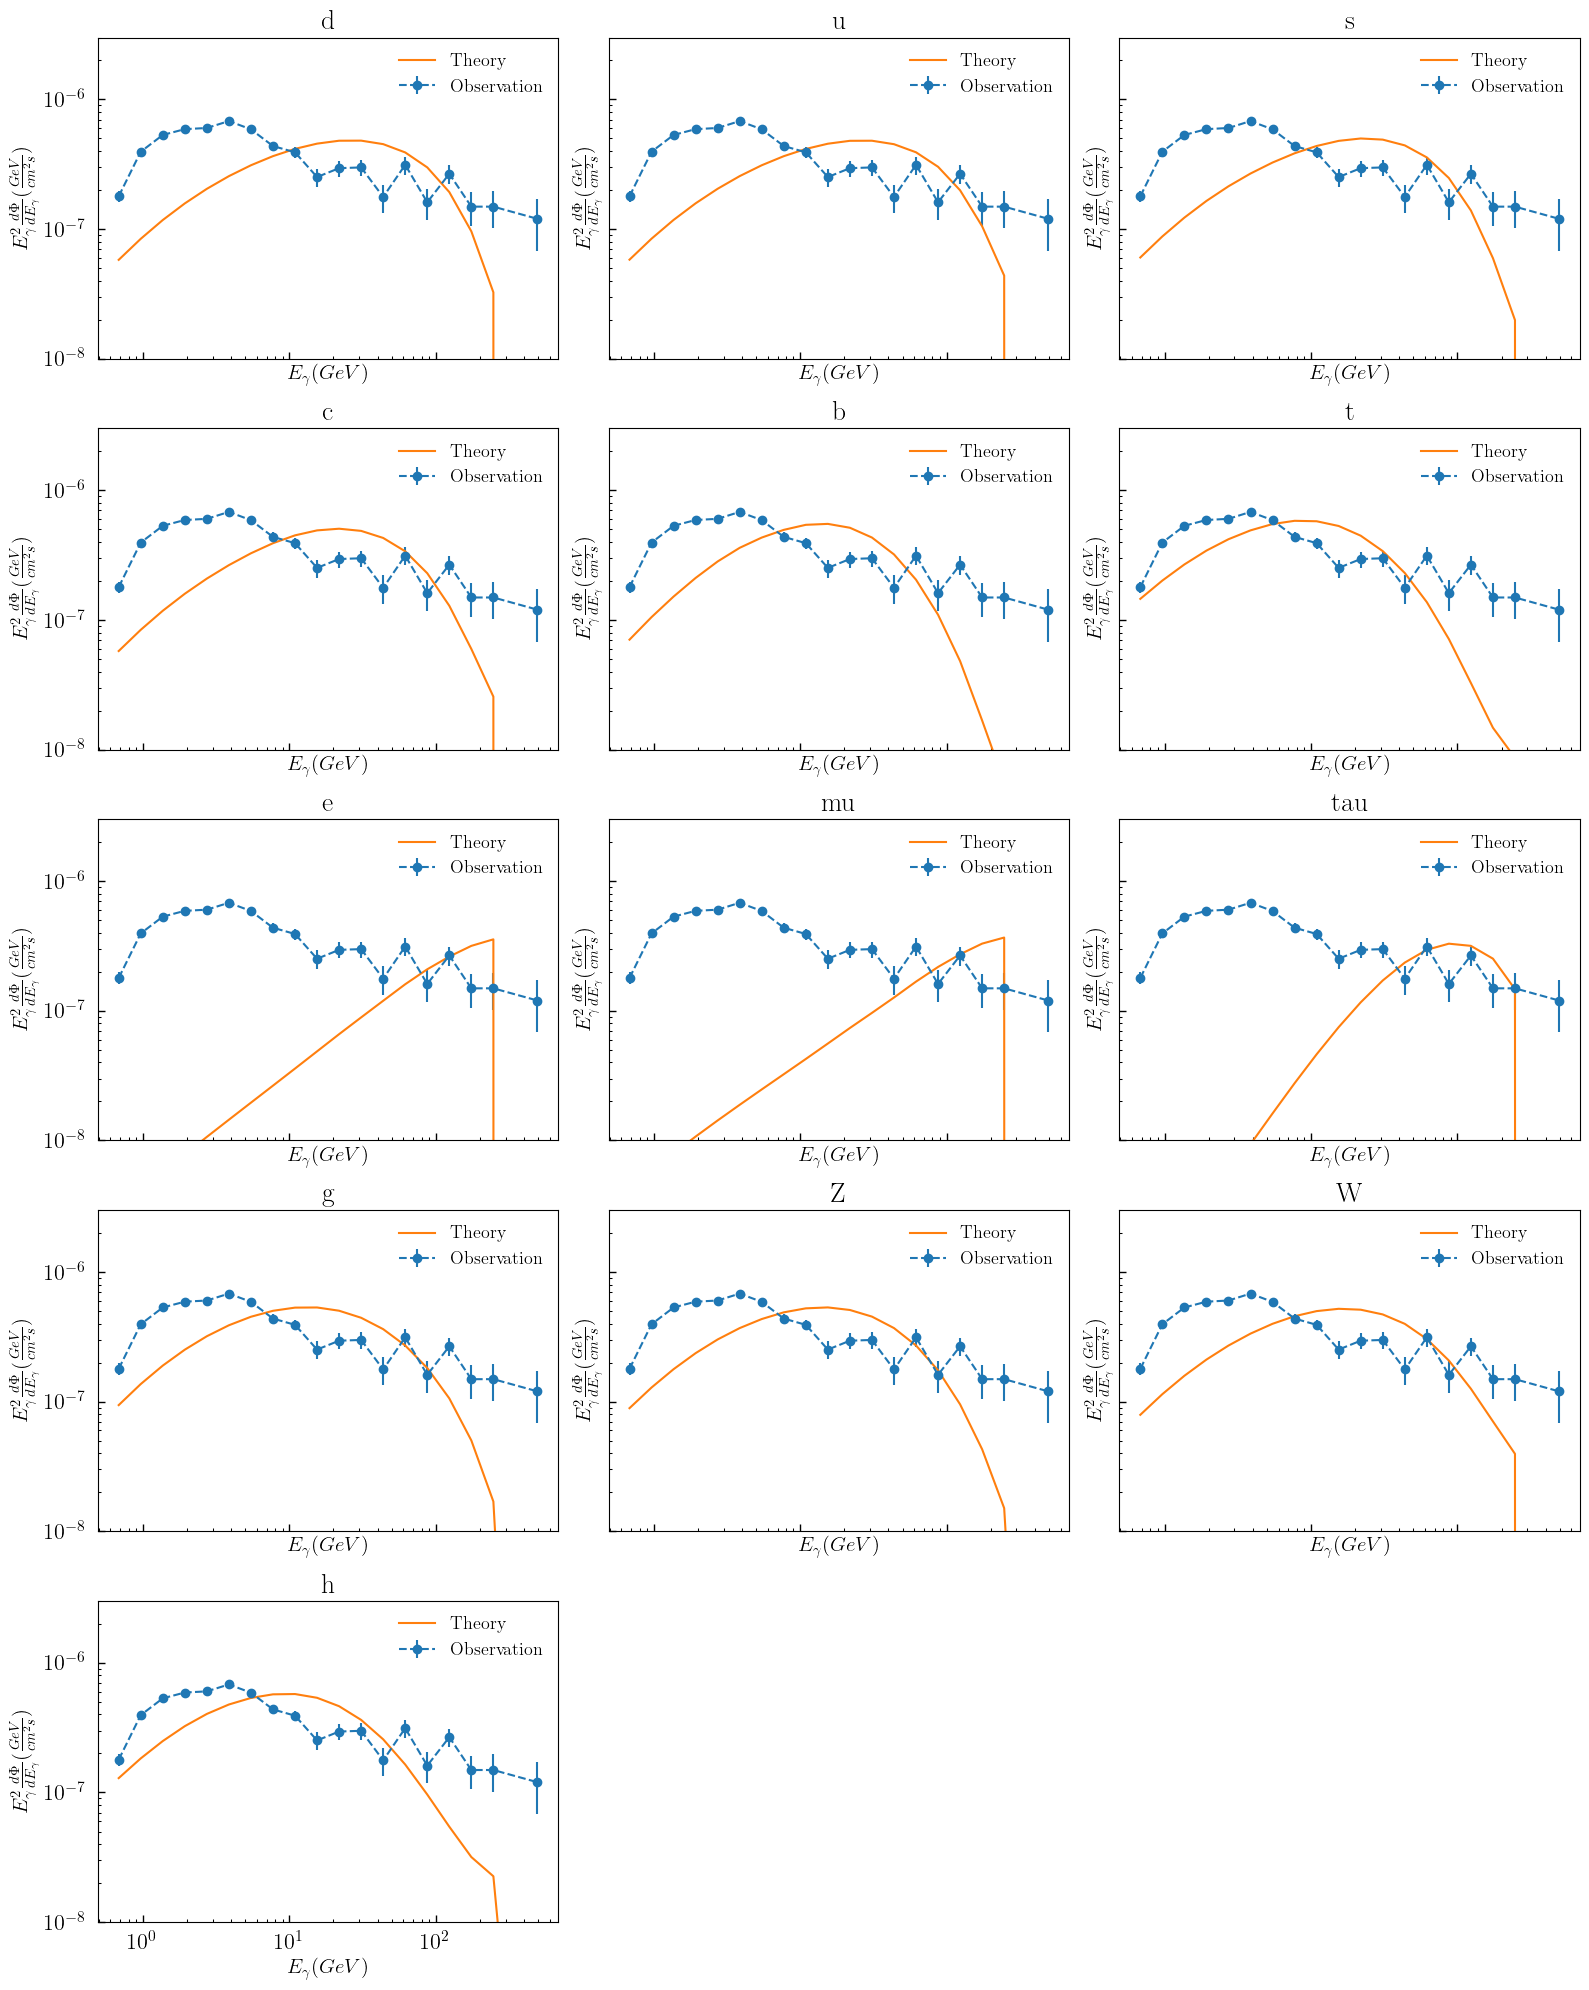
\includegraphics[width=\linewidth]{images/best fit not all no unknow astronomy parameter_2.png}
    \caption{The comparison of simulation and Fermi-LAT gamma-ray excess data points.}
    \label{fig: various DM}
\end{figure}
\newpage

\begin{figure}[h]
    \centering
    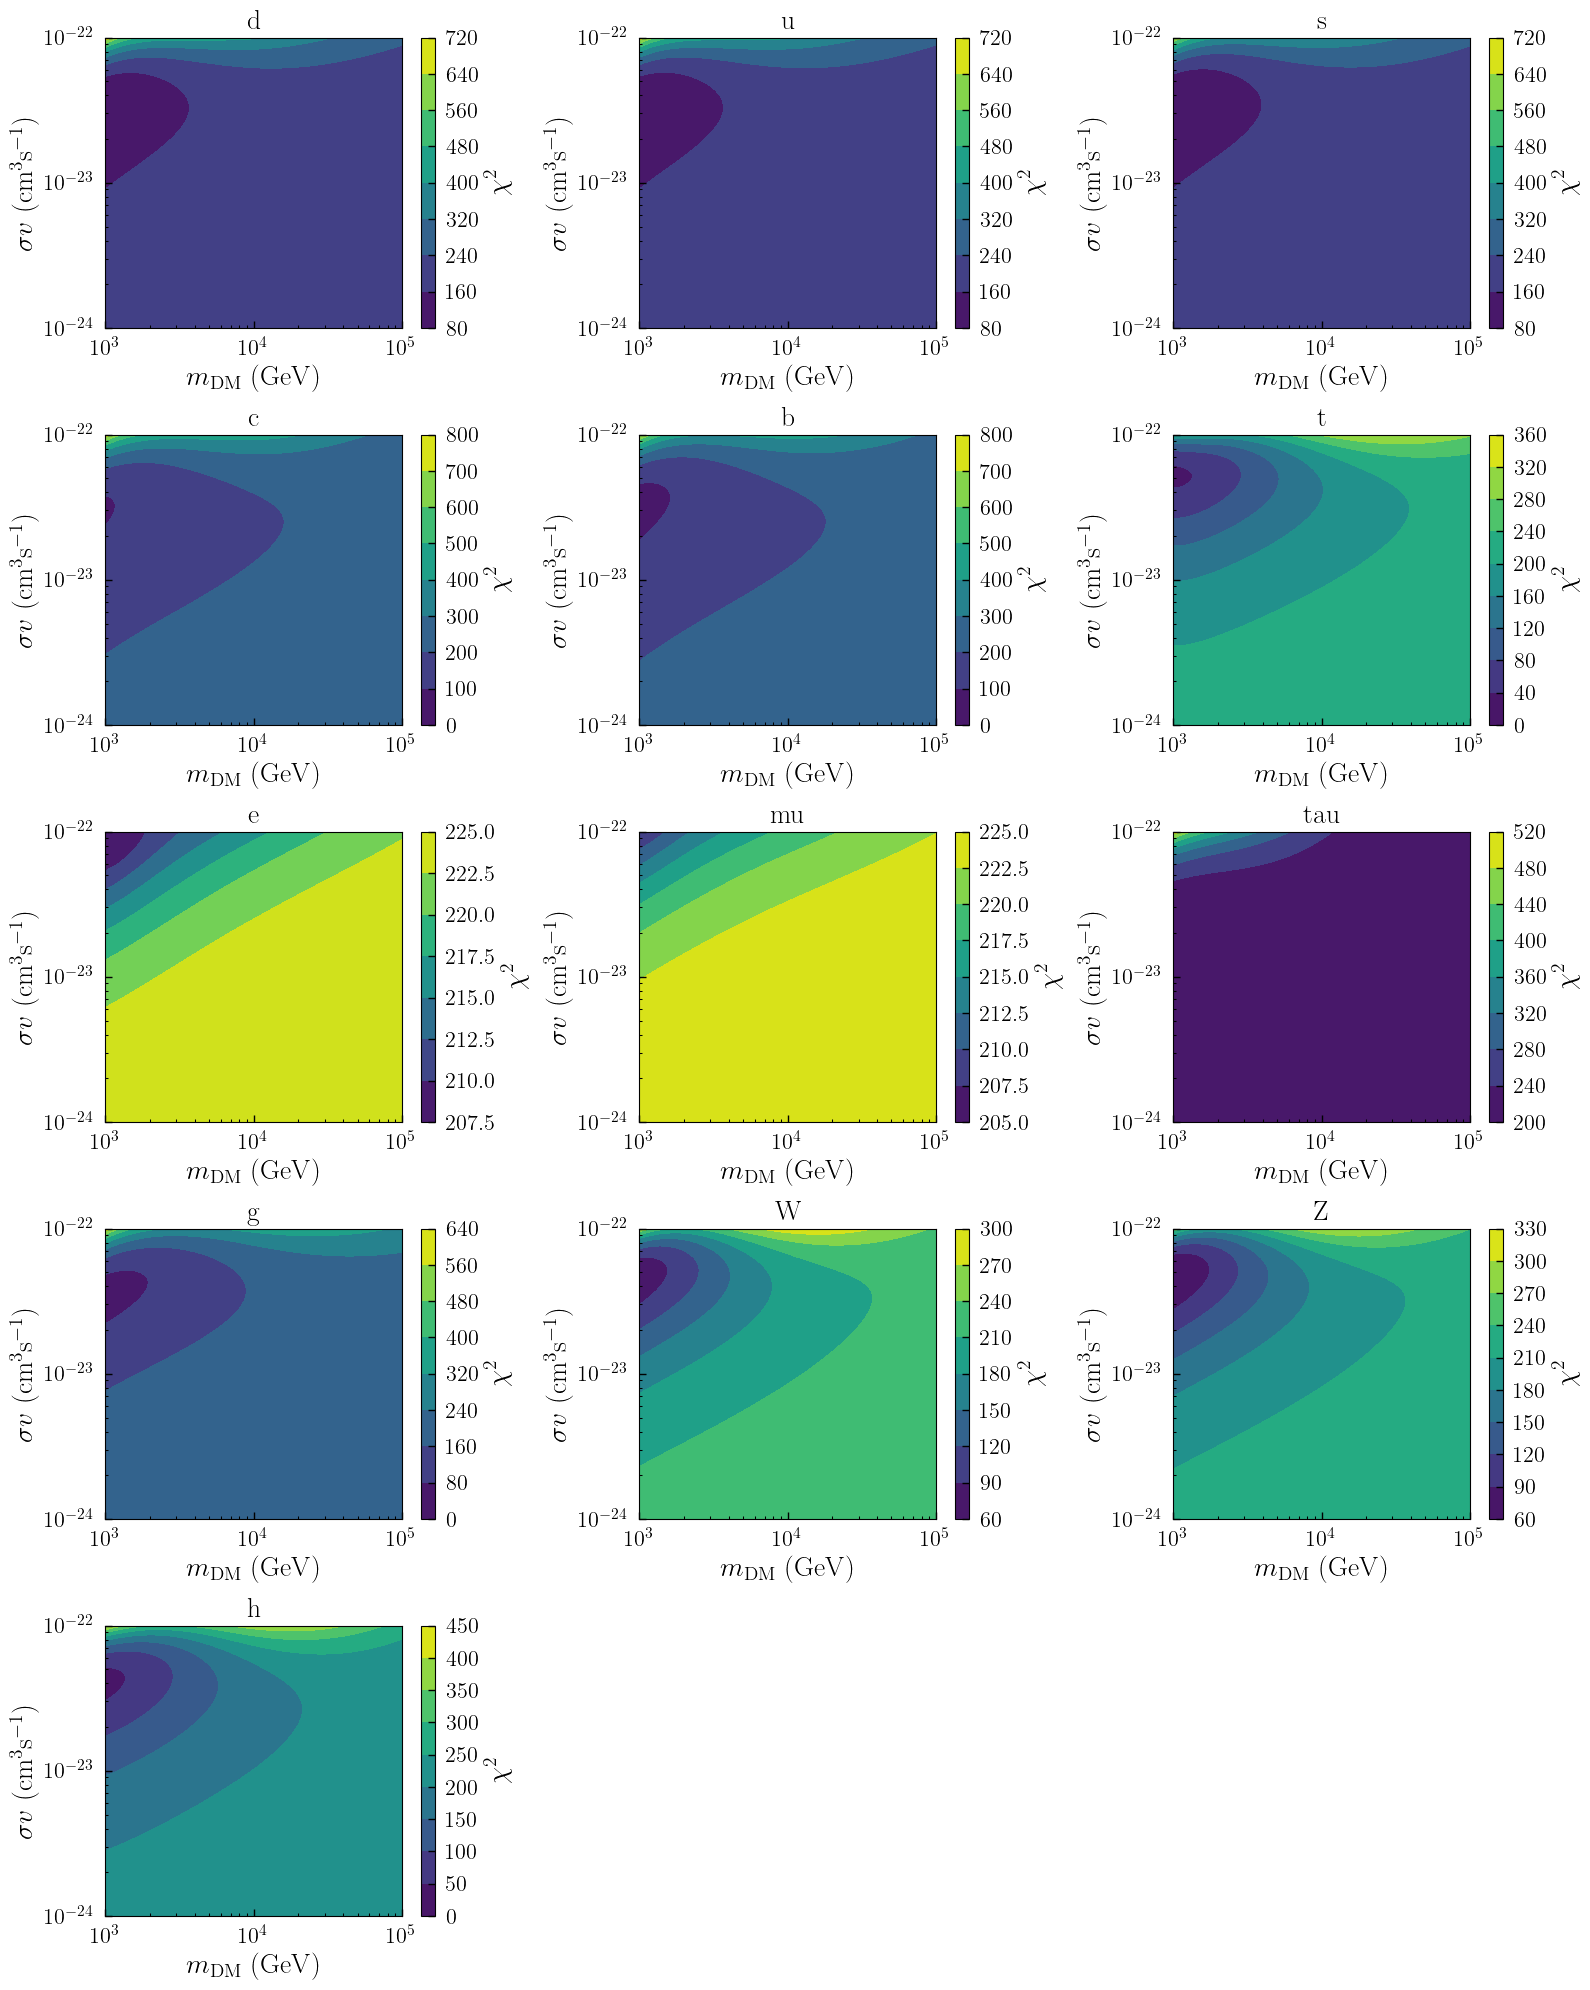
\includegraphics[width=\linewidth]{images/Contour_Best_Fit_not_all_2.png}
    \caption{The contour plot shows the chi-square value of quarks and bosons. The $x$-axis represents the mass of dark matter in the unit of TeV, and the $y$-axis represents the cross-section of the gamma-ray detected in the unit of cm$^3$/s.}
    \label{fig: contour}
\end{figure}

\FloatBarrier
\newpage

\section{Best-fit Graph and Contour Plot after putting the Unknown Astronomical Flux to the Simulation}

\begin{figure}[h]
    \centering
    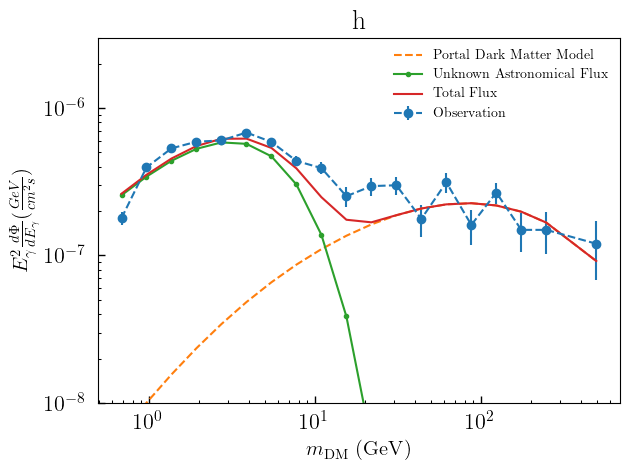
\includegraphics[width=0.5\linewidth]{images/partial_flux_3.png}
    \caption{Separation of spectrum lines of portal dark matter model and unknown astronomical flux.}
    \label{fig: partial flux}
\end{figure}

After the minimization method, the unknown astronomical flux, which has been added to the total flux of gamma-ray, we found the best-fit parameters, as shown in \autoref{tab: best fit unknown astronomy flux}. This time, the $m_\chi$ parameter does not shift to under TeV anymore and does stay in the range of this research consideration area.

A significant part of this research is the chi-square value. In \autoref{tab: best fit unknown astronomy flux}, it shows that the least chi-square value of every particle under consideration is about 4. In \autoref{fig:chi-square-table}, like the previous section, we use this table to perform the confidence test for population variance. This time, we have 5 parameters: $m_\chi, \langle \sigma v \rangle, N, \alpha$, and $E_{cut}$, by using \autoref{degree of freedom}, we have a degree of freedom equal to 14, which means the confidence of this chi-square at 99\% must be less than 4.66, which is every particle in \autoref{tab: best fit unknown astronomy flux}.

\begin{table}[h]
    \centering
    \begin{tabular}{|c|c|c|c|c|c|c|}
        \hline
        Particle & $m_\chi $(TeV) & $\langle\sigma v\rangle$ ($\times10^{-23}$ cm$^3$/s) & N ($\times10^{-7}$ GeV$^\alpha$) & $\alpha$ & E$_{cut}$ (GeV) & least $\chi^2$\\ \hline
        $d$ & 2.105 & 1.651 & 4.948 & -1.122 & 2.775 & 4.401\\
         $u$ & 1.918 & 1.649 & 4.946 & -1.142 & 2.699 & 4.342\\
         $s$ & 2.783 & 1.765 & 4.976 & -1.097 & 2.883 & 4.546\\
         $c$ & 3.054 & 1.639 & 4.999 & -1.089 & 2.933 & 4.607\\
         $b$ & 4.037 & 1.753 & 5.079 & -1.110 & 2.848 & 4.546\\
         $t$ & 6.428 & 2.253 & 5.020 & -1.149 & 2.682 & 4.212\\
         $e$ & 1.000 & 5.220 & 4.614 & -0.533 & 7.990 & 13.194\\
         $\mu$ & 1.000 & 8.883 & 4.607 & -0.548 & 7.694 & 12.906\\
         $\tau$ & 1.000 & 1.476 & 4.745 & -0.733 & 5.376 & 8.291\\
         $g$ & 6.136 & 1.982 & 5.083 & -1.140 & 2.710 & 4.284\\
         $Z$ & 3.511 & 2.360 & 5.001 & -1.134 & 2.739 & 4.263\\
         $W$ & 2.915 & 2.378 & 4.976 & -1.150 & 2.679 & 4.183\\
         $h$ & 4.642 & 1.977 & 5.058 & -1.161 & 2.643 & 4.271\\
         \hline
    \end{tabular}
    \caption{This table shows the best-fit parameters for quarks such as $d, u, s, c, b, t$ and bosons such as $g, Z, W, h$ with the least chi-square value from those parameters.}
    \label{tab: best fit unknown astronomy flux}
\end{table}

With those parameters shown in \autoref{tab: best fit unknown astronomy flux}, the plot of gamma-ray flux from the simulation and the unknown astronomical flux now seems to go along well, this provides us the confidence to trust that this result is the best-fit as shown in \autoref{fig: best-fit unknown astronomy flux}.

In the final part of this research, we have done the contour plot to show the constraint of dark matter mass, $m_\chi$, and cross-section, $\langle \sigma v \rangle$. The area labeled with color shows the value of chi-square value within the range of confidence level from 99\%, 95\%, and 90\% respectively from inside to outside of the contour as shown in \autoref{fig: contour unknown astronomy flux}.

\begin{figure}
    \centering
    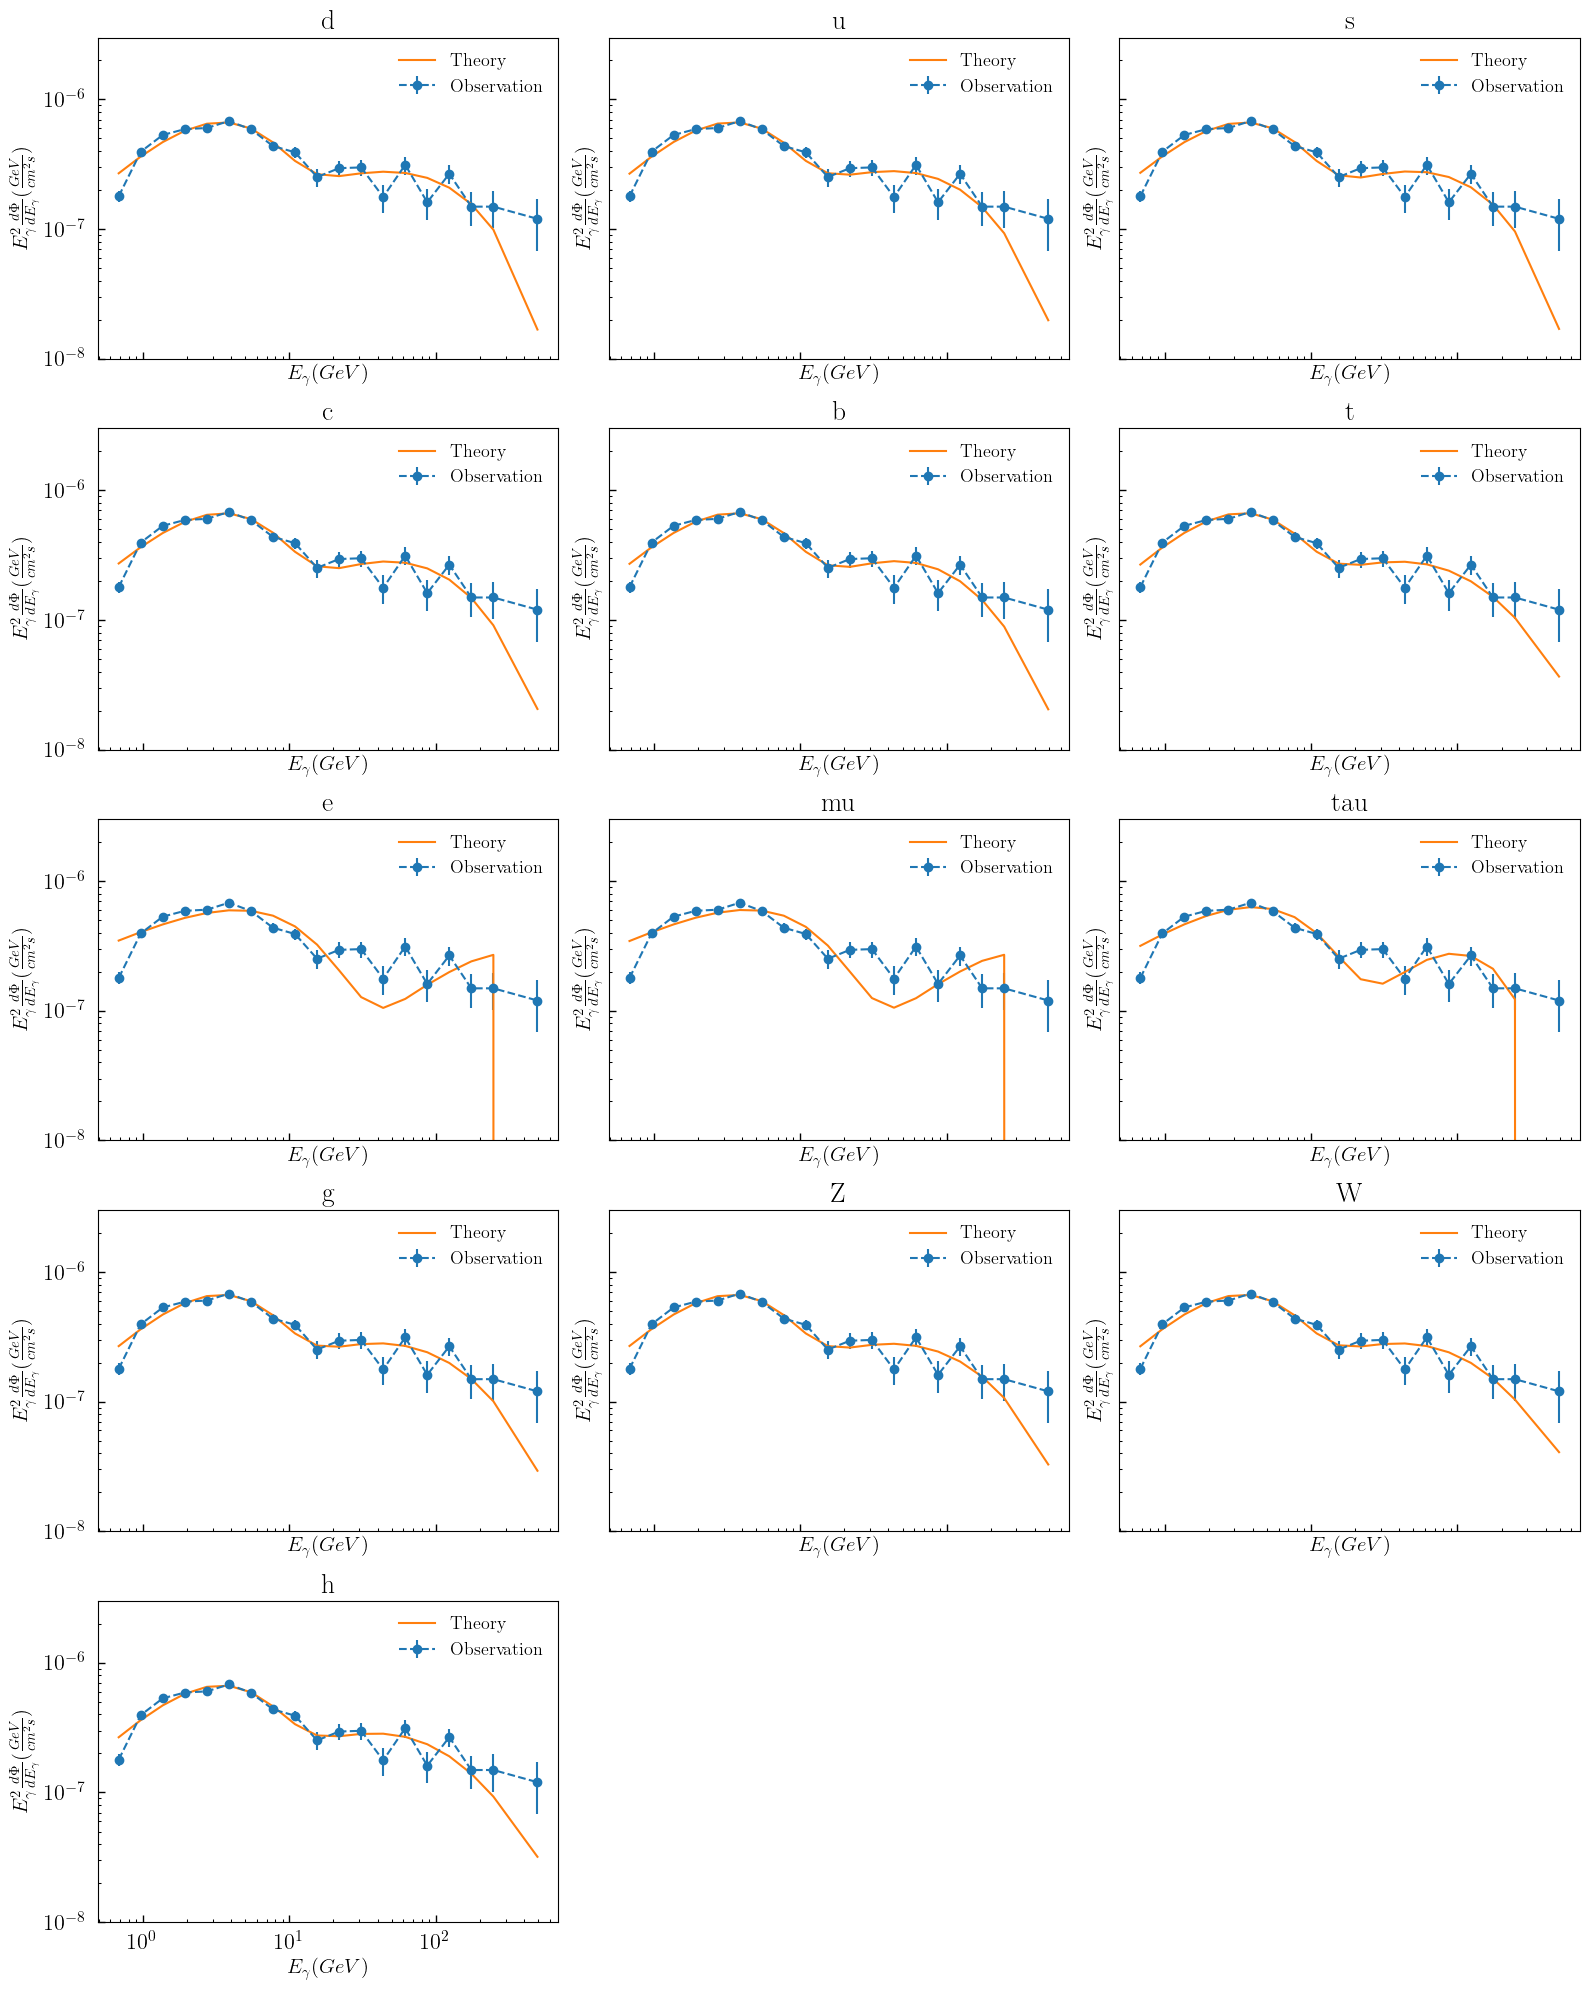
\includegraphics[width=\linewidth]{images/Best_fit_not_all_2.png}
    \caption{The comparison of simulation with additional unknown astronomical flux and Fermi-LAT data points.}
    \label{fig: best-fit unknown astronomy flux}
\end{figure}

\begin{figure}
    \centering
    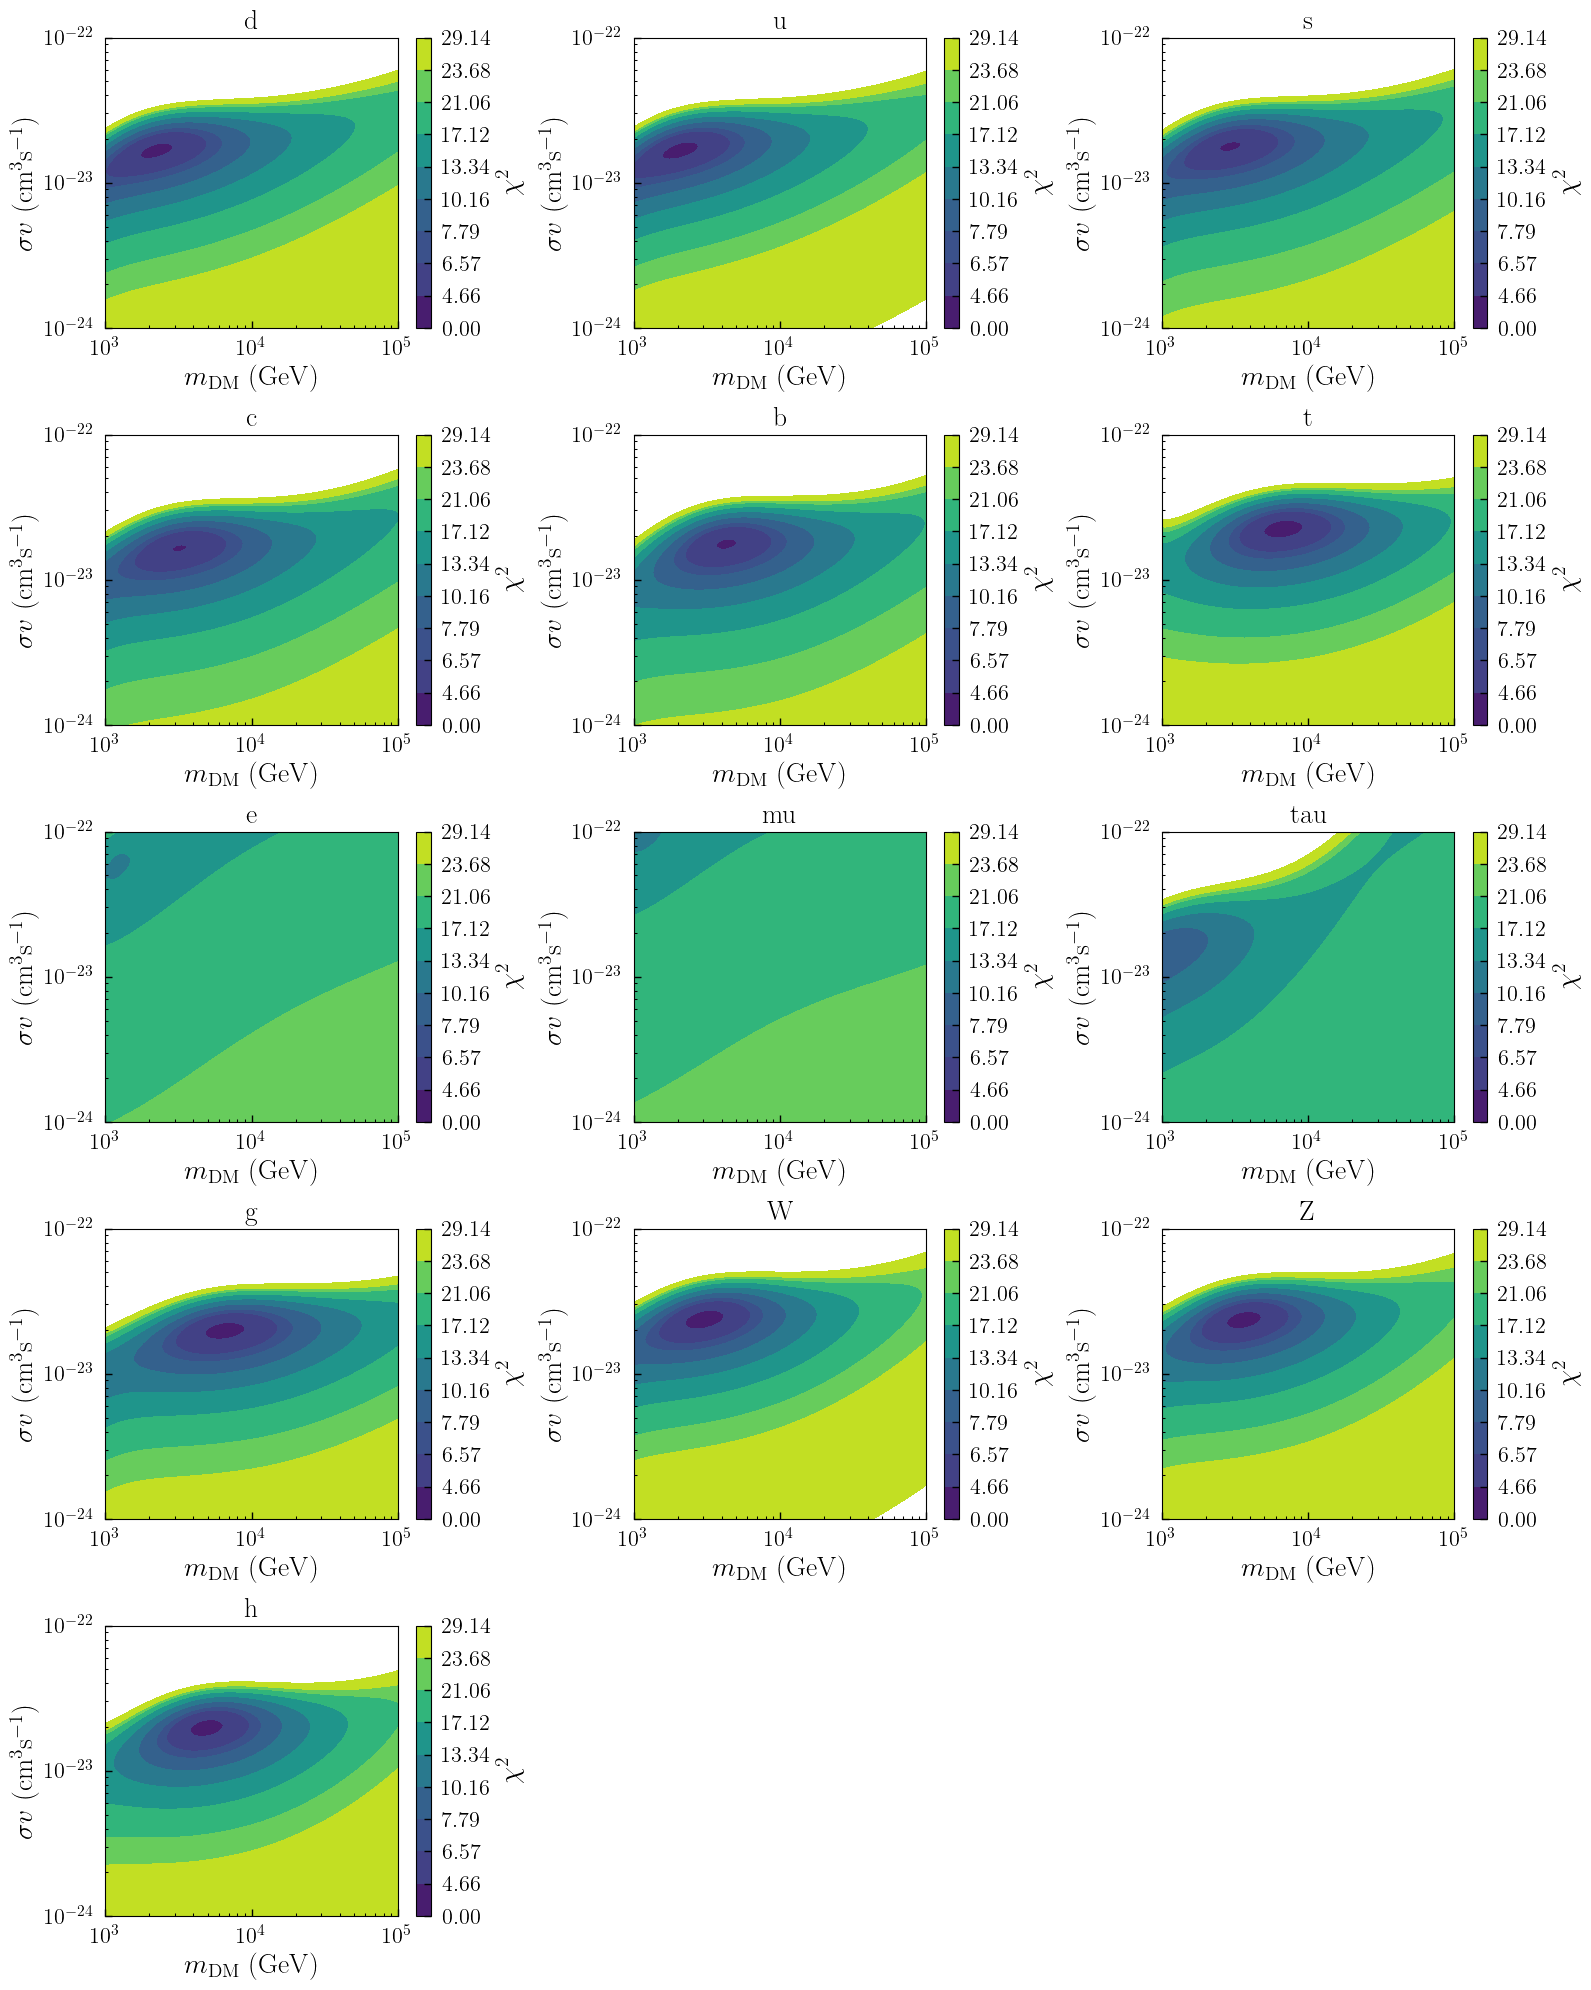
\includegraphics[width=\linewidth]{images/Contour_Best_Fit_not_all_3.png}
    \caption{The contour plot shows the chi-square value of quarks and bosons. The $x$-axis represents the mass of dark matter in the unit of TeV, and the $y$-axis represents the cross-section of the gamma-ray detected in the unit of cm$^3$/s. The chi-square value shown on the right side of each image represents the chi-square value of 4.66, 6.57, 7.79 means the confidence level of 99\%, 95\%, and 90\% respectively.}
    \label{fig: contour unknown astronomy flux}
\end{figure}


\chapter{Conclusion}
In this research, we focus on studying the gamma-ray flux produced by the dark matter annihilation phenomenon and comparing it with data points from the Fermi-LAT, which observed the flux of gamma-ray at the center of the Milky Way galaxy. The hypothesis we use in this work is that the gamma-ray flux observed from Fermi-LAT comes from the annihilation of dark matter, which produces another particle in the standard model, and that particle decays to gamma-ray and also may come from the unknown astronomical flux.

First of all, we need to find the number of gamma-ray produced from dark matter annihilation at an arbitrary mass. In this case, we use two Python codes: \textbf{\textit{CascadeSpectra}} from \cite{Marco_Cirelli_2011} and \textit{\textbf{HDMSpectra}} from \cite{Bauer_2021}. We use data from these two codes to find the number flux of gamma-rays varies from 0.5 GeV to 1000 TeV, and we pick only data points that have the same energy value as data points from Fermi-LAT. With those data, we know how many numbers of gamma-ray at specific gamma-ray energies are produced from dark matter annihilation at each mass of dark matter. In particular, we obtain the probability of finding gamma-ray per gamma-ray energy from various masses of dark matter, $dP/dE$.

The next part is to find the probability of finding the mediator particle per gamma-ray energy after the annihilation process, as shown in \autoref{complete dPdE}. After we substitute $dP/dE$ and \autoref{complete dPdE} into \autoref{dPhidE}, Finally we can find the flux of gamma-ray produced from dark matter annihilation, again as mentioned, both directly exert gamma-ray and from the decay of mediator particle.

Then what we have to do is compare the result we got from the \autoref{dPhidE} with the data points from Fermi-LAT. But in \autoref{dPhidE} has two arbitrary parameters we can freely pick, the mass of dark matter, $m_\chi$, and cross-section, $\langle \sigma v \rangle$. That is why we need to use \textit{minimization} to find the best-fit values of those two parameters. The method we use to clarify the distribution of data is \textit{reduced chi-square}. The result of using minimization and reduced chi-square to find best-fit parameters is shown in \autoref{tab: best fit} and plotted in \autoref{fig: various DM}. The value of reduced chi-square with two parameters $m_\chi$ and $\langle \sigma v \rangle$ is shown in \autoref{fig: contour}. Notice in \autoref{fig: various DM}, the spectra lines from the simulation are not consistent with the data points from Fermi-LAT at all, not only that, the value of chi-square value shown in \autoref{fig: contour} is too high when compared to \autoref{fig:chi-square-table} with the degree of freedom 17. This tells us that something is missing, obviously gamma-ray flux.

The result we shown in \autoref{tab: best fit} does not seem to have a high confidence level, since in the last column, least $\chi^2$ is too high to be trusted followed \autoref{fig:chi-square-table} with the degree of freedom is 17. To make the result better, we need to remind again that our hypothesis again, we declares that the flux observed from Fermi-LAT comes from the dark matter annihilation phenomenon and may come from an unknown astronomical flux. We use the unknown astronomical flux as an additional flux to fulfill the missing part of the result.

To find the unknown astronomical flux value, we can use \autoref{unknown astronomy flux equation} which has three parameters as described already in the methodology. Again, we use the \textit{minimization} and the \textit{reduced chi-square} to find best-fit parameters, this time we have five parameters, $m_\chi$, $\langle \sigma v \rangle$, $N$, $\alpha$, and $E_{cut}$, which mean the degree of freedom is 13. The result of the simulation with the addition of an unknown astronomical flux is shown in \autoref{tab: best fit unknown astronomy flux}. Notice in \autoref{fig: best-fit unknown astronomy flux}, spectra lines from the simulation are consistent with data points from Fermi-LAT, not only that, the contour plot shown in \autoref{fig: contour unknown astronomy flux}. As shown in \autoref{fig: contour unknown astronomy flux}, the chi-square value is impressive because it is under the trusted of data with 99\%, 95\%, and 90\%. The exceptional case concerns leptons such as electrons, muons, and tauons. According to the trend in \autoref{tab: best fit unknown astronomy flux}, these particles are likely to produce gamma-ray when they are below the TeV scale.

The best result we found is the W-boson with the parameters of $m_\chi=2.915$ TeV, $\langle \sigma v \rangle=2.378\times 10^{-23}$ cm$^3$/s, $N=4.976\times 10^{-7}$ GeV$^\alpha, \alpha=-1.150$, and $E_{cut}=2.679$ GeV, the least chi-square value is 4.271.

The result of this work reviews the trend of dark matter mass beyond the TeV scale. It gives us the confidentiality of using \textbf{\textit{HDMSpectra}} to reproduce gamma-ray from the dark matter pair annihilation process.

\bibliography{references}
\bibliographystyle{plain}

\newpage

\appendix
\chapter{Derivation of J-factor Distance}
From \autoref{Rmw}, we can rearrange the equation, so we obtain
\begin{eqnarray*}
    R_{MW}^2 &=& R^2_{sc} + l^2_{max} - 2R_{sc}l_{max}\cos\left(\psi\right)\\
    0 &=& R^2_{sc} + l^2_{max}-2R_{sc}l_{max}\cos\left(\psi\right) - R_{MW}^2.\\
\end{eqnarray*}
Then we use the completing square method.
\begin{eqnarray*}
    0 &=& R^2_{sc} + l^2_{max} - 2R_{sc}l_{max}\cos\left(\psi\right)-R_{MW}^2 + R_{sc}^2\cos^2(\psi) - R_{sc}^2\cos^2(\psi)\\
    &=& R^2_{sc} -R_{MW}^2 + l^2_{max} - 2R_{sc}l_{max}\cos\left(\psi\right) + R_{sc}^2\cos^2(\psi) - R_{sc}^2\cos^2(\psi)\\
    &=& R^2_{sc} - R_{MW}^2 + (l_{max} - R_{sc}\cos(\psi))^2 - R_{sc}^2\cos(\psi).\\
\end{eqnarray*}
We notice the $R_{sc}^2\cos(\theta)$ term has the ability to perform a Pythagorean identity.
\begin{eqnarray*}
   0 &=& R^2_{sc} - R_{MW}^2 + (l_{max} - R_{sc}\cos(\psi))^2 - R_{sc}^2\cos(\psi) - R_{sc}^2\sin^2(\psi) + R_{sc}^2\sin^2(\psi)\\
    &=& R^2_{sc} - R_{MW}^2 + (l_{max} - R_{sc}\cos(\psi))^2 - R_{sc}^2 + R_{sc}^2\sin^2(\psi)\\
    &=& (l_{max} - R_{sc}\cos(\psi))^2 - R_{MW}^2 + R_{sc}^2\sin^2(\psi).\\
\end{eqnarray*}
At this step, we can find the farthest distance of the dark matter annihilation phenomenon in the Milky Way by rearranging this equation again.
\begin{eqnarray*}
    (l_{max} - R_{sc}\cos(\psi))^2 &=& R_{MW}^2 - R_{sc}^2\sin^2(\psi)\\
    l_{max} - R_{sc}\cos(\psi) &=& \sqrt{R_{MW}^2 - R_{sc}^2\sin^2(\psi)}\\
    l_{max} &=& \sqrt{R_{MW}^2-R_{sc}^2\sin^2(\psi)}+R_{sc}\cos(\psi).
\end{eqnarray*}

%\chapter{Programming process flowchart}
%\begin{figure}
%    \centering
%    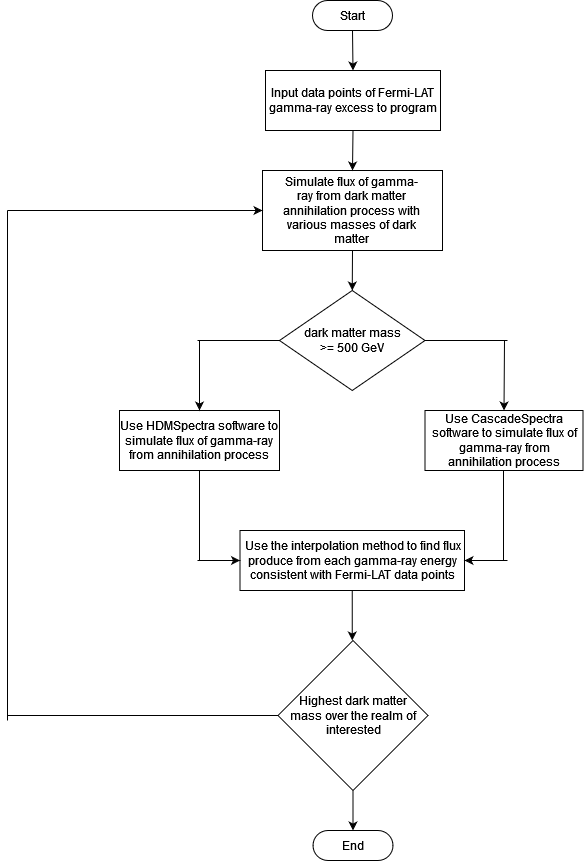
\includegraphics[width=0.5\linewidth]{dPdE_gamma.png}
%\end{figure}


\chapter{Program Codes}
\section{Declare Modules}
\begin{python}
# Load HDMSpectra
from HDMSpectra import HDMSpectra

# Import numpy
import numpy as np

# Import scipy
from scipy import integrate, interpolate, optimize


# Import DataFrame
import pandas as pd

# Import memory clear module
import gc


# Plotting defaults
import matplotlib.pyplot as plt
import matplotlib as mpl
mpl.rcParams['text.usetex'] = True
mpl.rcParams['font.family'] = 'serif'
mpl.rcParams['xtick.labelsize'] = 16
mpl.rcParams['ytick.labelsize'] = 16
mpl.rcParams['xtick.major.size'] = 5
mpl.rcParams['xtick.minor.size'] = 2.5
mpl.rcParams['xtick.major.width'] = 1.0
mpl.rcParams['xtick.minor.width'] = 0.75
mpl.rcParams['xtick.major.pad'] = 8
mpl.rcParams['xtick.direction'] = 'in'
mpl.rcParams['ytick.major.size'] = 5
mpl.rcParams['ytick.minor.size'] = 2.5
mpl.rcParams['ytick.major.width'] = 1.0
mpl.rcParams['ytick.minor.width'] = 0.75
mpl.rcParams['ytick.major.pad'] = 8
mpl.rcParams['ytick.direction'] = 'in'
mpl.rcParams['legend.fontsize'] = 13
mpl.rcParams['legend.frameon'] = False
plt.rcParams['axes.titlesize'] = 20
plt.rcParams['axes.labelsize'] = 20

cm = plt.get_cmap('jet')
\end{python}

\section{Read Datas from Fermi-LAT}
\begin{python}
fermi = pd.read_csv("fermi_excess_reduced.csv")
Ebin = fermi['Ebin'].to_numpy()
obs = fermi['obs'].to_numpy()
down_err = fermi['down_err'].to_numpy()
up_err = fermi['up_err'].to_numpy()
\end{python}

\section{Distribution of Dark Matter in the Galaxy}
\subsection{Dark Matter Density}
\begin{python}
NFW = lambda r,rs=24.42,rhos=0.184: rhos*(rs/r)*((1 + (r/rs))**-2)
Ein = lambda r,alpha=0.17,rs=28.44,rhos=0.033: rhos*np.exp((-2/alpha)*(((r/rs)**alpha) - 1))
EinB = lambda r,alpha=0.11,rs=35.24,rhos=0.021: rhos*np.exp((-2/alpha)*(((r/rs)**alpha) - 1))
Iso = lambda r,rs=4.38,rhos=1.387: rhos/(1 + (r/rs)**2)
Burkert = lambda r,rs=12.67,rhos=0.712: rhos/((1 + r/rs)*(1 + (r/rs)**2))
Moore = lambda r,rs=30.28,rhos=0.105: rhos*(rs/r)**1.16 * (1 + r/rs)**-1.84

NFW_list = []
Ein_list = []
EinB_list = []
Iso_list = []
Burkert_list = []
Moore_list = []
for r in np.arange(10**-3,10**2,10**-3):
  NFW_list.append(NFW(r))
  Ein_list.append(Ein(r))
  EinB_list.append(EinB(r))
  Iso_list.append(Iso(r))
  Burkert_list.append(Burkert(r))
  Moore_list.append(Moore(r))

r = np.arange(10**-3,10**2,10**-3)
plt.plot(r,NFW_list,label="NFW")
plt.plot(r,Ein_list,label="Einasto")
plt.plot(r,EinB_list,label="EinastoB")
plt.plot(r,Iso_list,label="Isothermol")
plt.plot(r,Burkert_list,label="Burkert")
plt.plot(r,Moore_list,label="Moore")
plt.xscale("log")
plt.yscale("log")
plt.legend()
plt.title("Dark Matter Density")

plt.xlabel('r (kpc)')
plt.ylabel(r'$\rho_{DM} (GeV/cm^3)$')
plt.grid("true")
plt.tight_layout()
plt.show()
\end{python}

\subsection{J-factors}
\begin{python}
Rsc = 8.33 #kpc
rhosc = 0.47 #GeV/cm^3
Rmw = 26.8 #kpc

psi = []
NFW_list = []
Ein_list = []
EinB_list = []
Iso_list = []
Burkert_list = []
Moore_list = []
integral = []

J = lambda f: integrate.quad(f,0,lmax)[0]
r = lambda l: np.sqrt(Rsc**2 + l**2 - 2*Rsc*l*np.cos(np.radians(i)))
NFW = lambda l,rs=24.42,rhos=0.184: rhos*(rs/r(l))*((1 + (r(l)/rs))**-2)
Ein = lambda l,alpha=0.17,rs=28.44,rhos=0.033: rhos*np.exp((-2/alpha)*(((r(l)/rs)**alpha) - 1))
EinB = lambda l,alpha=0.11,rs=35.24,rhos=0.021: rhos*np.exp((-2/alpha)*(((r(l)/rs)**alpha) - 1))
Iso = lambda l,rs=4.38,rhos=1.387: rhos/(1 + (r(l)/rs)**2)
Burkert = lambda l,rs=12.67,rhos=0.712: rhos/((1 + r(l)/rs)*(1 + (r(l)/rs)**2))
Moore = lambda l,rs=30.28,rhos=0.105: rhos*(rs/r(l))**1.16 * (1 + r(l)/rs)**-1.84

n = 180 #degree unit
delta = 0.1
for i in np.arange(1,n + 1,delta):
  lmax = np.sqrt(Rmw**2 - (Rsc**2)*np.sin(np.radians(i))) + Rsc*np.cos(np.radians(i))
  psi.append(i)
  NFW_list.append(J(NFW))
  Ein_list.append(J(Ein))
  EinB_list.append(J(EinB))
  Iso_list.append(J(Iso))
  Burkert_list.append(J(Burkert))
  Moore_list.append(J(Moore))

integrated_J_NFW = integrate.simpson(NFW_list, dx=delta)
integrated_J_Ein = integrate.simpson(Ein_list, dx=delta)
integrated_J_EinB = integrate.simpson(EinB_list, dx=delta)
integrated_J_Iso = integrate.simpson(Iso_list, dx=delta)
integrated_J_Burkert = integrate.simpson(Burkert_list,dx=delta)
integrated_J_Moore = integrate.simpson(Moore_list, dx=delta)
integrated = [integrated_J_NFW,integrated_J_Ein,integrated_J_EinB,integrated_J_Iso,integrated_J_Burkert,integrated_J_Moore]

plt.plot(psi,NFW_list,label="NFW")
plt.plot(psi,Ein_list,label="Ein")
plt.plot(psi,EinB_list,label="EinB")
plt.plot(psi,Iso_list,label="Isothermol")
plt.plot(psi,Burkert_list,label="Burkert")
plt.plot(psi,Moore_list,label="Moore")
plt.yscale("log")
plt.legend()
plt.grid("true")
plt.tight_layout()
plt.xlabel(r'$\theta (^\circ)$')
plt.ylabel(r'$J(\theta)$')
plt.title('J-factors')
plt.show()
\end{python}

\section{CascadeSpectra + HDMSpectra}
\subsection{dNdE function}
\begin{python}
# Define dNdE as a functional
def dNdE(mDM, initialstate):
    # If mass is less than 500 GeV then u, d, s defined as q

    if mDM < 500:   # CascadeSpectra
        filename = 'CascadeSpectra/Spectra/AtProduction_gammas.dat' # CascadeSpectra

        # Annihilation process
        with open(filename) as f:
            lines = (line for line in f if not line.startswith('#'))
            data = np.genfromtxt (lines, names = True ,dtype = None)

        massvals = data["mDM"]
        index = np.where(np.abs( (massvals - mDM) / mDM) < 1.e-3)
        xvals = 10**(data["Log10x"][index]) # x = E/mDM

        flux = data[initialstate][index]/(np.log(10)*xvals)
        loadspec = interpolate.interp1d(xvals,flux)
        def dNdx(x):
            fluxval = loadspec(x)
            if (x>1 or fluxval<0):
                return 0
            else:
                return fluxval

        E = mDM*xvals
        dNdE = [(1/mDM)*dNdx(x) for x in xvals]

    else:   # HDMSpectra
        data = 'HDMSpectra-master/data/HDMSpectra.hdf5' # location of hdf5 file

        x = np.logspace(-4.,0.,1000) # Energy fraction values, x = 2E/mDM

        # Extract the spectrum using HDMSpectra.spec
        dNdx = HDMSpectra.spec(22, initialstate, x, mDM, data, annihilation=True)

        E = x*mDM/2
        dNdE = dNdx*2/mDM # Since E and dNdx are fixed, it's mean the dNdE will decrease per incresing of mDM

    return E, dNdE
\end{python}

\subsection{Selected dark matter mass}
\begin{python}
# Find mDM that > E_gamma for every E_gamma in Ebin
test_mDM = ([5, 6, 8, 10, 300, 330, 360, 400, 450]
          + [*range(30, 150 + 10, 10)]
          + [*range(160, 280 + 20, 20)]
          + [*range(500, 950 + 50, 50)]
          + [*range(1000, 1000*1000 + 100, 100)]) # mDM from 5 GeV to 1000 TeV
test_mDM.sort()

DM_mass =[]
for i in range(len(Ebin)):
    list = []
    for j in range(len(test_mDM)):
        if Ebin[i] > test_mDM[j]:
            list.append(0)
        else:
            list.append(test_mDM[j])
    DM_mass.append(list)

print(len(DM_mass[0]))
\end{python}

\subsection{dPdE\_gamma}
\begin{python}
# Declare 2 variable for mass < 500 GeV, and > 500 GeV
particles_5 = ['q','q','q','c','b','t','e','nue','mu','numu','tau','nutau','g','gamma','Z','W','h']
particles_500 = ['d','u','s','c','b','t','e','nue','mu','numu','tau','nutau','g','gamma','Z','W','h']

for i in range(len(particles_500)):
    print(particles_500[i])
    list = []
    for j in range(len(Ebin)):
        sub_list = []
        for k in range(len(DM_mass[0])):

            if DM_mass[j][k] == 0:
                sub_list.append(0)
            elif DM_mass[j][k] < 500:
                E, dPdE = dNdE(DM_mass[j][k], particles_5[i])
                interp = np.interp(Ebin[j], E, dPdE)
                sub_list.append(interp)
            elif DM_mass[j][k] >= 500:
                E, dPdE = dNdE(DM_mass[j][k], particles_500[i])
                interp = np.interp(Ebin[j], E, dPdE)
                sub_list.append(interp)

        list.append(sub_list)
    df = pd.DataFrame(list)
    df.to_csv('dPdE_gamma_new/{}.csv'.format(particles_500[i]), header=DM_mass[0], index=False)
    gc.collect()

# W boson return 0 value for some x which give negative values
# Well, I would say it's make my work a lot easier, great job HDMSpectra
\end{python}

\section{Portal Dark Matter Model}
\subsection{Emin \& Emax}
\begin{python}
# Define constant
particles = ['d','u','s','c','b','t','e','nue','mu','numu','tau','nutau','g','gamma','Z','W','h']
mj = [0.0047, 0.0022, 0.096, 1.28, 4.18, 173.1, 0.000511, 0.000001, 0.10566, 0.00017, 1.7768, 0.0182, 0, 0, 91.19, 80.36, 124.97] # GeV, I get it from Wikipedia
#mDM = np.arange(1*1000, 1000*1000 + 1000, 1000)   # From 5 TeV to 1000 TeV
mDM = np.logspace(3, 5, 100)

# Calculate E_min & E_max for each mediator(phi)
E_mediator_min = []
E_mediator_max = []
for i in range(len(mj)): # N of particles I consider
    list_min = []
    list_max = []
    for j in range(len(mDM)):  # declare that I will use mDM from 1TeV to 1000TeV
        m_mediator = mDM[j]/2
        lambda_phi = np.sqrt(1 - (m_mediator/mDM[j])**2)
        lambda_j = np.sqrt(1 - (2*mj[i]/m_mediator)**2)
        list_min.append((mDM[j]/2)*(1 - lambda_phi*lambda_j))
        list_max.append((mDM[j]/2)*(1 + lambda_phi*lambda_j))
    E_mediator_min.append(list_min)
    E_mediator_max.append(list_max)

\end{python}

\subsection{dPdE\_mediator}
\begin{python}
dPdE_mediator = []
for i in range(len(mj)):
    #print('j:',particles[i])
    list = []
    for j in range(len(mDM)):
        sublist = []
        for k in range(len(Ebin)):
            #print('j:', particles[i], ', Ebin:', Ebin[j], ', mDM:', DM_mass[k])
            m_mediator = mDM[j]/2
            #print((1 - (m_mediator/DM_mass[k])**2), (1 - (2*mj[i]/m_mediator)**2), (1 - 2*Ebin[j]/DM_mass[k])**2)
            dPdE_m = ((4/(np.pi*mDM[j]))
                     *np.sqrt(abs((1 - (m_mediator/mDM[j])**2)*(1 - (2*mj[i]/m_mediator)**2) - (1 - 2*Ebin[k]/mDM[j])**2))
                     /((1 - (m_mediator/mDM[j])**2)*(1 - (2*mj[i]/m_mediator)**2)))
            sublist.append(dPdE_m)
        list.append(sublist)
    dPdE_mediator.append(list)
\end{python}

\subsection{dNdE}
\begin{python}
# Declare particles name
#particles = ['d','u','s','c','b','t','e','nue','mu','numu','tau','nutau','g','gamma','Z','W','h']

dNdE_DM = []
for i in range(len(particles)):
    print(particles[i])
    list = []
    dPdE_gamma = pd.read_csv('dPdE_gamma/{}.csv'.format(particles[i])).to_numpy()
    for j in range(len(mDM)):
        sublist = []
        for k in range(len(Ebin)):
            #limit = np.linspace(E_mediator_min[i][j], E_mediator_max[i][j], len(dPdE_gamma[k]))
            #integrated = integrate.simpson(dPdE_gamma[k] * dPdE_mediator[i][j][k], limit)
            intpl = interpolate.CubicSpline(DM_mass[0] ,dPdE_gamma[k])
            integrated = integrate.quad(intpl, E_mediator_min[i][j], E_mediator_max[i][j])[0]
            #integrated = simpsons_rule(dPdE_gamma[k] * dPdE_mediator[i][j][k], E_mediator_min[i][j], E_mediator_max[i][j], 1000)
            sublist.append(2 * integrated)
        list.append(sublist)
    dNdE_DM.append(list)

    np.save('dNdE_DM.npy', dNdE_DM)
\end{python}

\section{$d\Phi/dE_\gamma$}
\subsection{Find the best-fit cross-section}
\begin{python}
dNdE_DM = np.load('dNdE_DM.npy')

# Define dPhidE function
def E2dPhidE_func(E, sv):
    Rsc = 8.33  # kpc
    rhosc = 0.47  # GeV/cm^3
    J = integrated_J_NFW  # Make sure to define or replace with the appropriate value
    return E**2 * 3.085677581e15 * sv / (8 * np.pi) * (Rsc * rhosc**2) / mDM[m]**2 * J * dNdE_DM[p][m]

p_member = [0,1,2,3,4,5,12,14,15,16]
best_fit_ = []
for p in p_member:
    chi_min = float('inf')
    for m in range(len(mDM)):
        popt1, pcov1 = optimize.curve_fit(E2dPhidE_func, Ebin, obs)
        chi = chi2(obs, E2dPhidE_func(Ebin, *popt1))
        if chi < chi_min:
            chi_min = chi
            a = m
            b = popt1
    print(chi_min, mDM[a], b)
    #print('{}, chi2: {:,.3f}, m: {:,.3f} GeV, sv: {:,.3e}'.format(particles[p], chi_min, mDM[a], b))
    best_fit_.append([a, b])
\end{python}

\subsection{Plot the best-fit graph without the unknown astronomical source}
\begin{python}
def total_flux():
    Rsc = 8.33 #kpc
    rhosc = 0.47 #GeV/cm^3
    J = integrated_J_NFW
    m = best_fit_[p_member.index(p)][0]
    sv = best_fit_[p_member.index(p)][1]
    return Ebin**2 * 3.085677581*1e15 * sv/(8*np.pi) * (Rsc * rhosc**2)/mDM[m]**2 * J * [y for y in dNdE_DM[p][m]]


# Calculate the number of required rows and columns based on the number of particles
num_particles = 10
num_rows = num_particles // 3 + int(num_particles % 3 > 0)  # Ceiling division
num_cols = min(num_particles, 3)

# Set up subplots
fig, axs = plt.subplots(nrows=num_rows, ncols=num_cols, figsize=(12, 4 * num_rows), sharex=True, sharey=True)

for p in p_member:
    row = p_member.index(p) // 3  # Determine the row based on the floor division
    col = p_member.index(p) % 3  # Determine the column based on the modulo operation
    axs[row, col].set_title(f'{particles[p]}')

    axs[row, col].errorbar(Ebin, obs, yerr=[down_err, up_err], label='Observation', linestyle='--', marker='o')

    total = total_flux()
    axs[row, col].plot(Ebin, total, label='Theory')

    # Optionally add legend to each subplot
    axs[row, col].set_xlabel(r'$E_\gamma$', size=15)
    axs[row, col].set_ylabel(r'$E_\gamma^2\frac{d\Phi}{dE_\gamma}$', size=15)
    axs[row, col].set_xscale('log')
    axs[row, col].set_yscale('log')
    axs[row, col].set_ylim([1e-8, 0.3e-5])
    axs[row, col].legend()

# Remove empty subplots
for i in range(num_particles, num_rows * num_cols):
    fig.delaxes(axs.flatten()[i])

plt.tight_layout()
plt.show()
\end{python}

\subsection{Find the Reduced chi-square value}
\begin{python}
# Define dPhidE function
def E2dPhidE_func(dNdE, sv):
    Rsc = 8.33 #kpc
    rhosc = 0.47 #GeV/cm^3
    J = integrated_J_NFW
    return Ebin**2 * 3.085677581*1e15 * sv/(8*np.pi) * (Rsc * rhosc**2)/mDM[m]**2 * J * dNdE[m]


# Define the reduced-chisquare function
def chi2(y_obs, y_exp):
    residuals = y_obs - y_exp
    error = down_err
    chisquare = np.sum((residuals/error)**2)
    dof = len(obs) - 2 # Number of parameters
    reduced_chisquare = chisquare/dof
    return reduced_chisquare

chi_min = float('inf')

SV = np.logspace(-24, -22, len(mDM))

for p in range(len(particles)):
    list = []
    for m in range(len(mDM)):
        sublist = []
        for sv in SV:
            x = E2dPhidE_func(dNdE_DM[p], sv)
            chi = chi2(obs, x)
            sublist.append(chi)
        list.append(sublist)
    Chi2DataFrame = pd.DataFrame(list)
    Chi2DataFrame.to_csv('Chi2/{}.csv'.format(particles[p]), header=SV, index=False)
\end{python}

\subsection{Plot the contour of chi-square value}
\begin{python}
# Create subplots for each particle
fig, axes = plt.subplots(nrows=len(particles)//4 + 1, ncols=4, figsize=(16, 3 * (len(particles)//4 + 1)))

for i, particle in enumerate(particles):
    row = i // 4  # Determine the row based on the floor division
    col = i % 4  # Determine the column based on the modulo operation
    Chi2 = pd.read_csv('Chi2/{}.csv'.format(particle)).to_numpy()
    Chi2 = np.transpose(Chi2)

    # Plot the contour plot in the i-th subplot
    cs = axes[row, col].contourf(mDM, SV, Chi2)
    axes[row, col].set_title(f'{particle}')
    axes[row, col].set_xlabel(r'$m_{\mathrm{DM}} \ (\mathrm{GeV})$')
    axes[row, col].set_ylabel(r'$\sigma v \ (\mathrm{cm^3 s^{-1}})$')
    axes[row, col].set_xscale('log')
    axes[row, col].set_yscale('log')
    fig.colorbar(cs, ax=axes[row, col], label=r'$\chi^2$')

# Remove empty subplots
for i in range(len(particles), (len(particles)//4 + 1) * 4):
    fig.delaxes(axes.flatten()[i])

# Adjust layout to prevent overlapping
fig.tight_layout()
plt.show()
\end{python}

\section{Minimization Optimized}
\subsection{Find the best-fit parameters with the unknown astronomical source}
\begin{python}
# Define combined function
def combination(x, sv, N, alpha, Ecut):
    Rsc = 8.33 #kpc
    rhosc = 0.47 #GeV/cm^3
    J = integrated_J_NFW
    return N * x**(-alpha) * np.exp(-x/Ecut) + x**2 * 3.085677581*1e15 * sv/(8*np.pi) * (Rsc * rhosc**2)/mDM[m]**2 * J * [y for y in dNdE_DM[p][m]]

# Define the reduced-chisquare function
def chi2(y_obs, y_exp):
    residuals = y_obs - y_exp
    error = down_err
    chisquare = np.sum((residuals/error)**2)
    dof = len(obs) - 5 # Number of parameters
    reduced_chisquare = chisquare/dof
    return reduced_chisquare


best_fit = []
for p in range(len(particles)):
    chi_min = float('inf')
    for m in range(len(mDM)):
        popt1, pcov1 = optimize.curve_fit(combination, Ebin, obs, maxfev=1000000000)
        chi = chi2(obs, combination(Ebin, *popt1))
        if chi < chi_min:
            chi_min = chi
            a = m
            b, c, d, e = popt1
    print('{}, chi2: {:,.3f}, m: {:,.3f} GeV, sv: {:,.3e}, N: {:,.3e}, alpha: {:,.3f}, Ecut: {:,.3f}'.format(particles[p], chi_min, mDM[a], b, c, d, e))
    best_fit.append([a, b, c, d, e])
\end{python}

\subsection{Plot the best-fit graph with the unknown astronomical source}
\begin{python}
def total_flux():
    Rsc = 8.33 #kpc
    rhosc = 0.47 #GeV/cm^3
    J = integrated_J_NFW
    m = best_fit[p][0]
    sv = best_fit[p][1]
    N = best_fit[p][2]
    alpha = best_fit[p][3]
    Ecut = best_fit[p][4]
    return N * Ebin**(-alpha) * np.exp(-Ebin/Ecut) + Ebin**2 * 3.085677581*1e15 * sv/(8*np.pi) * (Rsc * rhosc**2)/mDM[m]**2 * J * [y for y in dNdE_DM[p][m]]


# Calculate the number of required rows and columns based on the number of particles
num_particles = len(particles)
num_rows = num_particles // 4 + int(num_particles % 4 > 0)  # Ceiling division
num_cols = min(num_particles, 4)

# Set up subplots
fig, axs = plt.subplots(nrows=num_rows, ncols=num_cols, figsize=(16, 4 * num_rows), sharex=True, sharey=True)

for p, particle in enumerate(particles):
    row = p // 4  # Determine the row based on the floor division
    col = p % 4  # Determine the column based on the modulo operation
    axs[row, col].set_title(f'{particles[p]}')

    axs[row, col].errorbar(Ebin, obs, yerr=[down_err, up_err], label='Observation', linestyle='--', marker='o')

    total = total_flux()
    axs[row, col].plot(Ebin, total, label = 'Theory')

    # Optionally add legend to each subplot
    axs[row, col].set_xlabel(r'$E_\gamma$', size=15)
    axs[row, col].set_ylabel(r'$E_\gamma^2\frac{d\Phi}{dE_\gamma}$', size=15)
    axs[row, col].set_xscale('log')
    axs[row, col].set_yscale('log')
    axs[row, col].set_ylim([1e-8, 0.3e-5])
    axs[row, col].legend()

# Remove empty subplots
for i in range(num_particles, num_rows * num_cols):
    fig.delaxes(axs.flatten()[i])

plt.tight_layout()
plt.show()
\end{python}

\subsection{Find the chi-square value of the parameters include the unknown astronomical source}
\begin{python}
# Define DM flux + astro flux function
def total_flux(dNdE, sv):
    Rsc = 8.33 #kpc
    rhosc = 0.47 #GeV/cm^3
    J = integrated_J_NFW
    N = best_fit[p][2]
    alpha = best_fit[p][3]
    Ecut = best_fit[p][4]
    return N * Ebin**(-alpha) * np.exp(-Ebin/Ecut) + Ebin**2 * 3.085677581*1e15 * sv/(8*np.pi) * (Rsc * rhosc**2)/mDM[m]**2 * J * dNdE[m]


# Define the reduced-chisquare function
def chi2(y_obs, y_exp):
    residuals = y_obs - y_exp
    error = down_err
    chisquare = np.sum((residuals/error)**2)
    dof = len(obs) - 5 # Number of parameters
    reduced_chisquare = chisquare/dof
    return reduced_chisquare


SV = np.logspace(-24, -20, len(mDM))


for p in range(len(particles)):
    print(particles[p])
    list = []
    for m in range(len(mDM)):
        sublist = []
        for sv in SV:
            chi = chi2(obs, total_flux(dNdE_DM[p],sv))
            sublist.append(chi)
        list.append(sublist)
    Chi2DataFrame = pd.DataFrame(list)
    Chi2DataFrame.to_csv('Chi2_total_flux/{}.csv'.format(particles[p]), header=SV, index=False)
\end{python}

\subsection{Plot the contour of parameters include the unknown astronomical source}
\begin{python}
levels = [0.0, 4.660, 6.571, 7.790]


# Create subplots for each particle
fig, axes = plt.subplots(nrows=len(particles)//4 + 1, ncols=4, figsize=(16, 3 * (len(particles)//4 + 1)))

for i, particle in enumerate(particles):
    row = i // 4  # Determine the row based on the floor division
    col = i % 4  # Determine the column based on the modulo operation
    Chi2_total = pd.read_csv('Chi2_total_flux/{}.csv'.format(particle)).to_numpy()
    Chi2_total = np.transpose(Chi2_total)

    # Plot the contour plot in the i-th subplot
    cs = axes[row, col].contourf(mDM, SV, Chi2_total, levels=levels)
    axes[row, col].set_title(f'{particle}')
    axes[row, col].set_xlabel(r'$m_{\mathrm{DM}} \ (\mathrm{GeV})$')
    axes[row, col].set_ylabel(r'$\sigma v \ (\mathrm{cm^3 s^{-1}})$')
    axes[row, col].set_xscale('log')
    axes[row, col].set_yscale('log')
    fig.colorbar(cs, ax=axes[row, col], label=r'$\chi^2$')

# Remove empty subplots
for i in range(len(particles), (len(particles)//4 + 1) * 4):
    fig.delaxes(axes.flatten()[i])

# Adjust layout to prevent overlapping
fig.tight_layout()
plt.show()

\end{python}

\end{document}